% Copyright 2004 by Till Tantau <tantau@users.sourceforge.net>.
%
% In principle, this file can be redistributed and/or modified under
% the terms of the GNU Public License, version 2.
%
% However, this file is supposed to be a template to be modified
% for your own needs. For this reason, if you use this file as a
% template and not specifically distribute it as part of a another
% package/program, I grant the extra permission to freely copy and
% modify this file as you see fit and even to delete this copyright
% notice. 

\documentclass{beamer}
\usepackage{graphicx}
\usepackage{breqn}
\graphicspath{ {./images/} }
\usepackage{amsmath}
\usepackage{dsfont}
\usepackage{ wasysym }
\usepackage[utf8]{inputenc}
\usepackage[T1]{fontenc}
\usepackage[backend=biber]{biblatex}
\bibliography{pres.bib}

% There are many different themes available for Beamer. A comprehensive
% list with examples is given here:
% http://deic.uab.es/~iblanes/beamer_gallery/index_by_theme.html
% You can uncomment the themes below if you would like to use a different
% one:
%\usetheme{AnnArbor}
%\usetheme{Antibes}
%\usetheme{Bergen}
%\usetheme{Berkeley}
\usetheme{Berlin}
%\usetheme{Boadilla}
%\usetheme{boxes}
%\usetheme{CambridgeUS}
%\usetheme{Copenhagen}
%\usetheme{Darmstadt}
%\usetheme{default}
%\usetheme{Frankfurt}
%\usetheme{Goettingen}
%\usetheme{Hannover}
%\usetheme{Ilmenau}
%\usetheme{JuanLesPins}
%\usetheme{Luebeck}
%\usetheme{Madrid}
%\usetheme{Malmoe}
%\usetheme{Marburg}
%\usetheme{Montpellier}
%\usetheme{PaloAlto}
%\usetheme{Pittsburgh}
%\usetheme{Rochester}
%\usetheme{Singapore}
%\usetheme{Szeged}
%\usetheme{Warsaw}

\title{Effects of Uncertainty in Heterogeneous Models}

% A subtitle is optional and this may be deleted
\subtitle{}

\author{Eric, Yannic and Andrian}
% - Give the names in the same order as the appear in the paper.
% - Use the \inst{?} command only if the authors have different
%   affiliation.

%\institute[Universities of Somewhere and Elsewhere] % (optional, but mostly needed)
%{
% \inst{1}%
%  Department of Computer Science\\
%  University of Somewhere
%  \and
%  \inst{2}%
%  Department of Theoretical Philosophy\\
%  University of Elsewhere}
% - Use the \inst command only if there are several affiliations.
% - Keep it simple, no one is interested in your street address.

\date{Project Module, 25.01.2017}
% - Either use conference name or its abbreviation.
% - Not really informative to the audience, more for people (including
%   yourself) who are reading the slides online

%\subject{Theoretical Computer Science}
% This is only inserted into the PDF information catalog. Can be left
% out. 

% If you have a file called "university-logo-filename.xxx", where xxx
% is a graphic format that can be processed by latex or pdflatex,
% resp., then you can add a logo as follows:

% \pgfdeclareimage[height=0.5cm]{university-logo}{university-logo-filename}
% \logo{\pgfuseimage{university-logo}}

% Delete this, if you do not want the table of contents to pop up at
% the beginning of each subsection:
\AtBeginSubsection[]
{
  \begin{frame}<beamer>{Outline}
    \tableofcontents[currentsection,currentsubsection]
  \end{frame}
}


% Let's get started
\begin{document}



\begin{frame}
  \titlepage
\end{frame}

\begin{frame}{Outline}
  \tableofcontents
  % You might wish to add the option [pausesections]
\end{frame}

% Section and subsections will appear in the presentation overview
% and table of contents.
\section{Idiosyncratic risk}
\subsection{}
\begin{frame}{Questions}
  \begin{itemize}
  
  \item {
How do changes in idiosynratic risk affect other economic variables in the long run? How do these results compare to an economy with complete markets? Are there distributional consequences?
  }

  \pause

  \item {
  We will look at changes in the unemployment benefit. 
  }
  
  \end{itemize}
\end{frame}




\begin{frame}{Model Summary}
  \begin{itemize}
  
  \item {
  Ex ante identical individuals are subject to uninsurable idiosyncratic shocks. 
  }
  \item {
Agents can interact on the asset market.
  }
  \item {
The model generates an endogenous distribution of wealth across consumers. 
  } 
  \item {
Aggregates and prices are jointly determined by the saving behavior of the collection of all households. 
}

  \end{itemize}

\end{frame}




\begin{frame}{Different parameters of the model}


  \centering{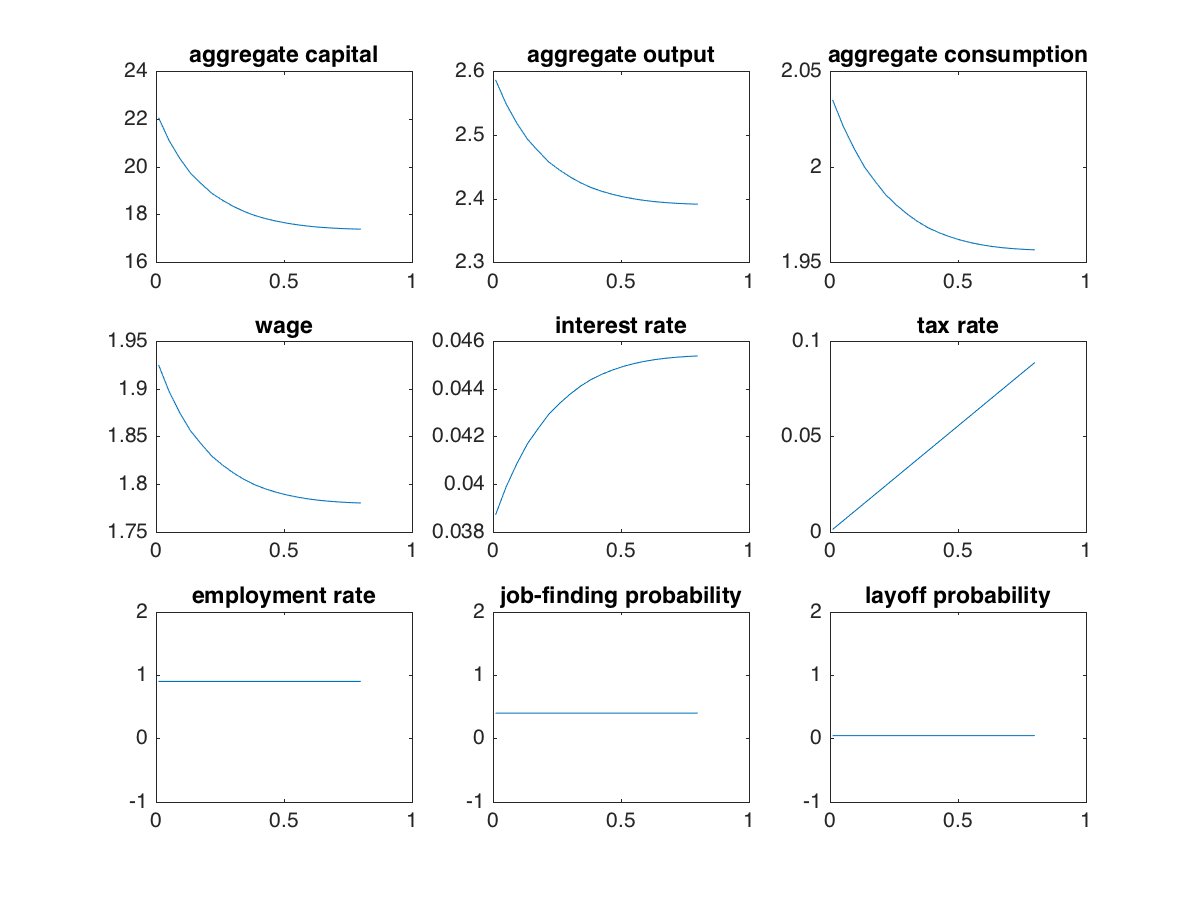
\includegraphics[scale=0.45]{parameters}}


\end{frame}

\begin{frame}{Different levels of risk aversion}


  \centering{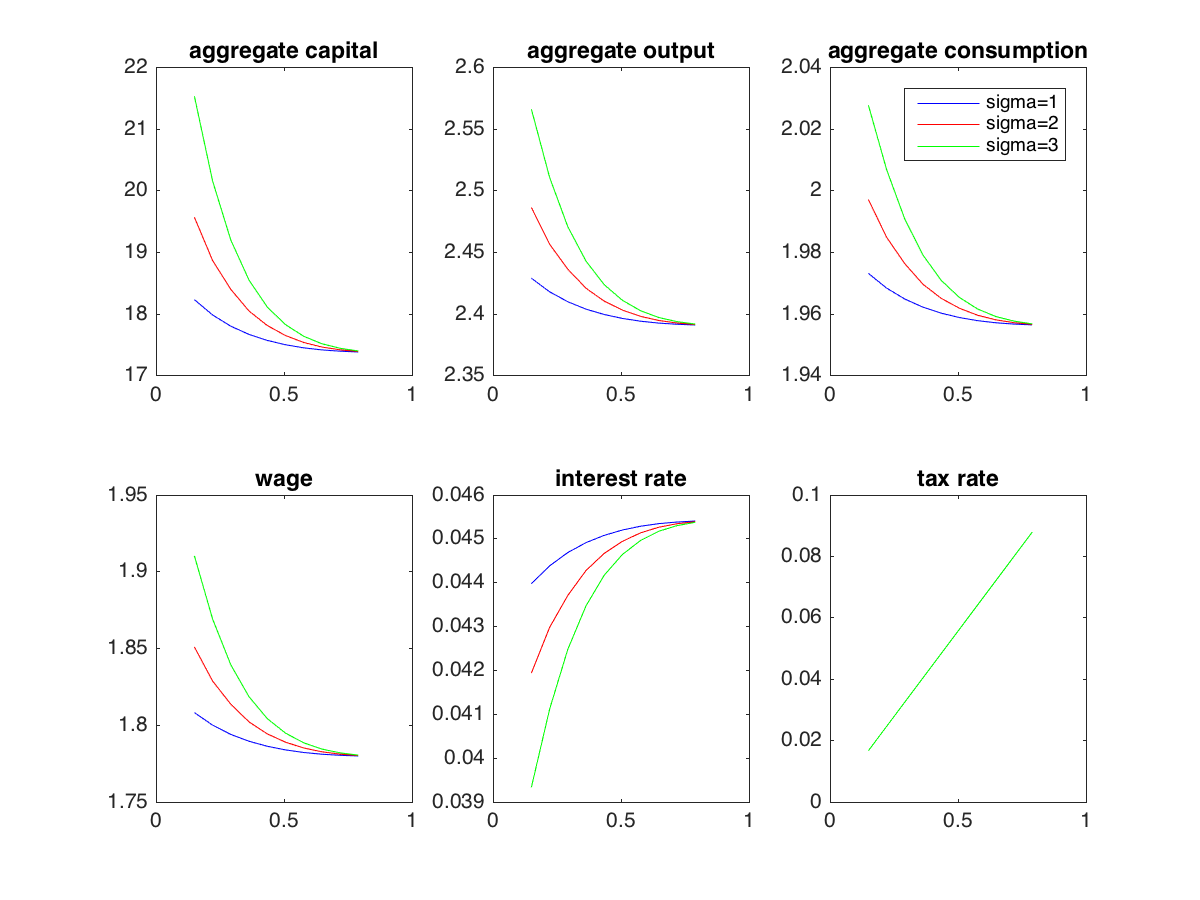
\includegraphics[scale=0.45]{parameters_sigma}}


\end{frame}


\begin{frame}{Comparing to complete markets}
  \begin{itemize}
  
 
    \item {
  How do the different levels of the aggregates compare to a situation with perfect insurance? 
  }

  \end{itemize}
  
\end{frame}
  

\begin{frame}{Comparing to complete markets}
  \centering{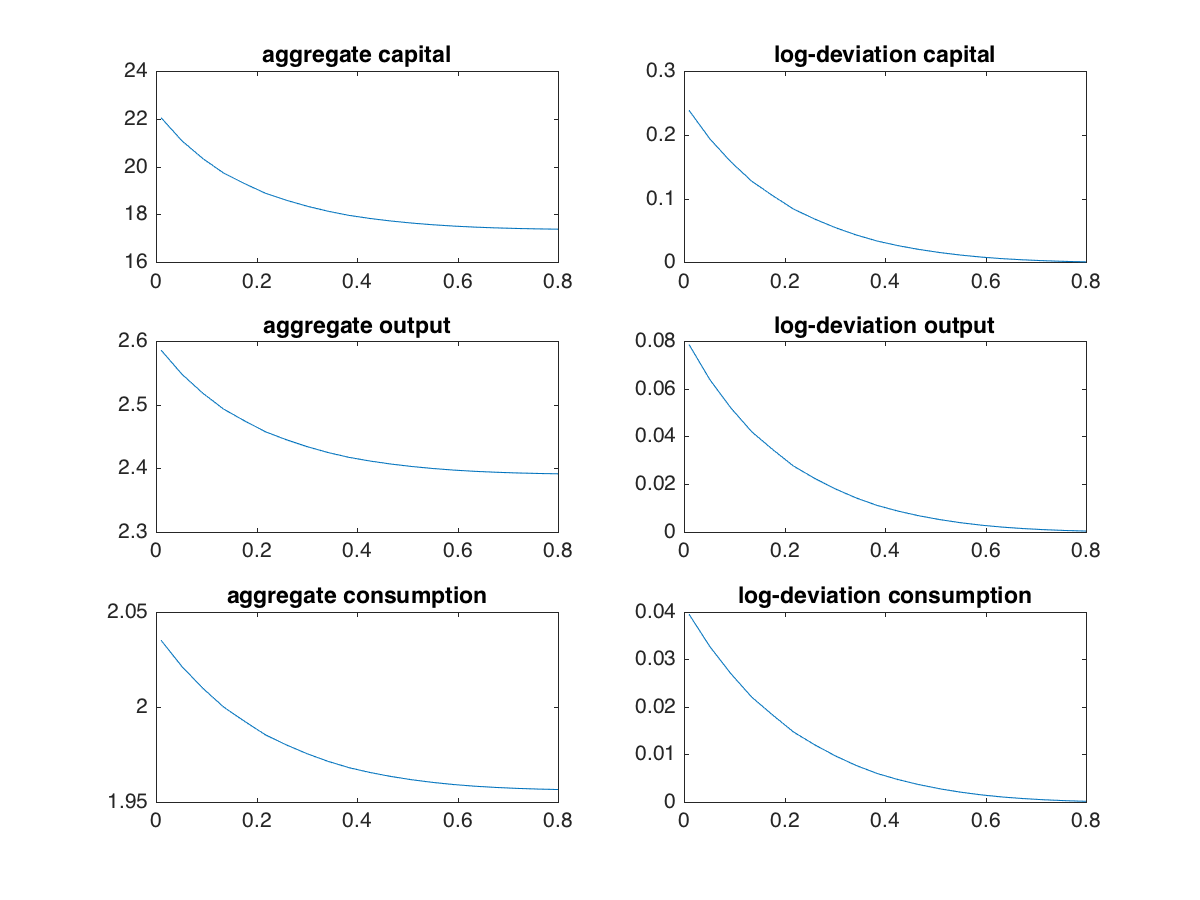
\includegraphics[scale=0.45]{log-deviation}}

\end{frame}
  
    
\begin{frame}{Comparing to complete markets}
  \begin{itemize}
  
  \item {
  As the insurance increases, the aggregates converge to the levels of the complete market economy. 
  }


  \end{itemize} 
\end{frame}



\begin{frame}{Distribution of capital}
 
\begin{figure}[!tbp]
  \centering
  \begin{minipage}[b]{0.325\textwidth}
    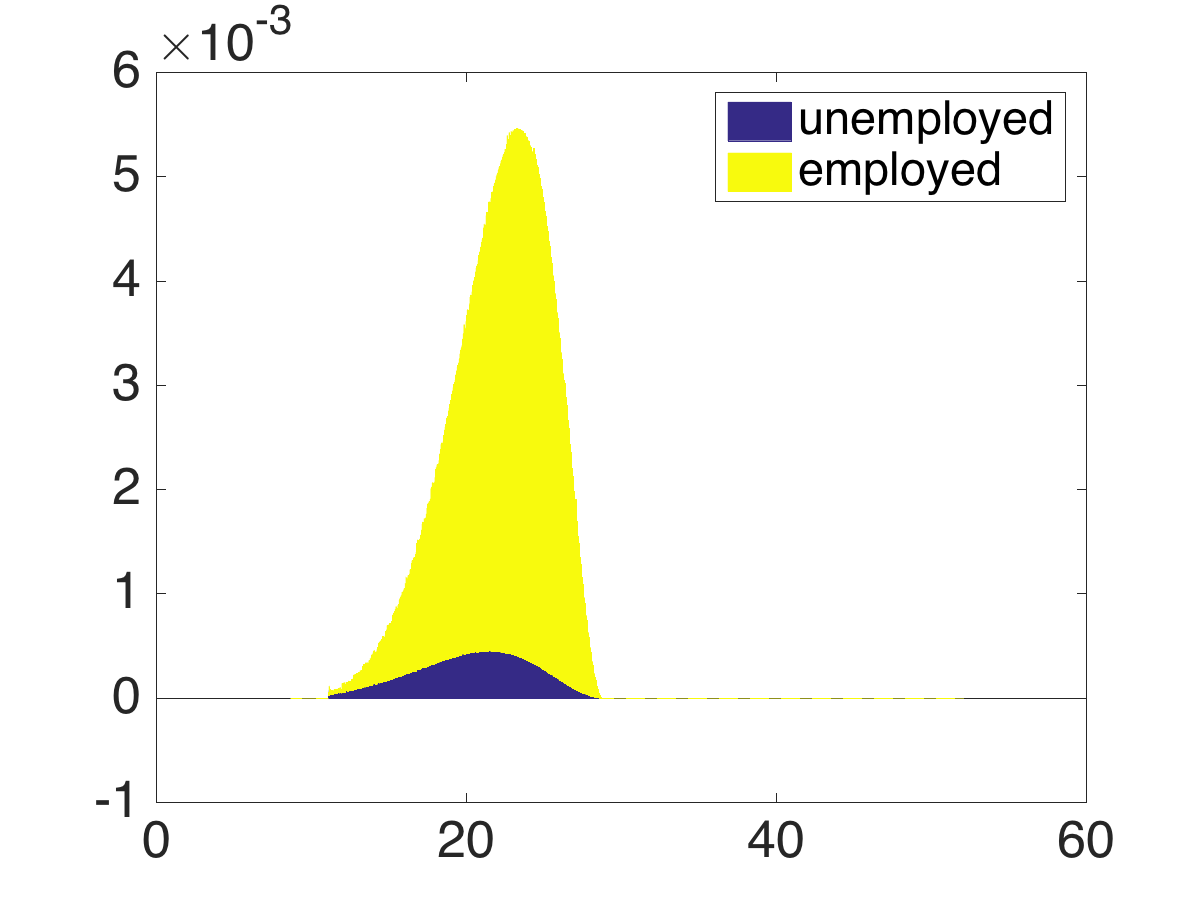
\includegraphics[width=\textwidth]{distribution1}
  \end{minipage}
  \hfill
  \begin{minipage}[b]{0.325\textwidth}
    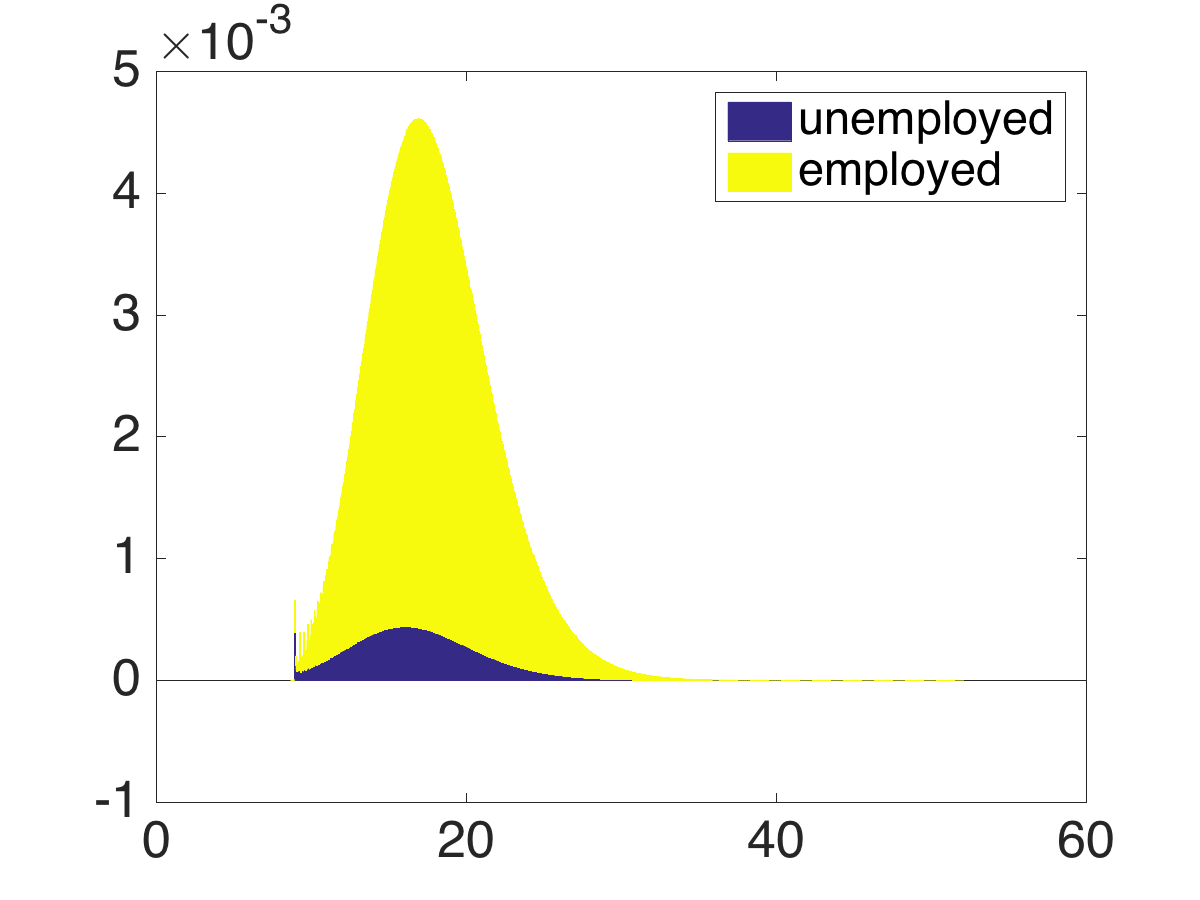
\includegraphics[width=\textwidth]{distribution2}
  \end{minipage}
  \hfill
  \begin{minipage}[b]{0.325\textwidth}
    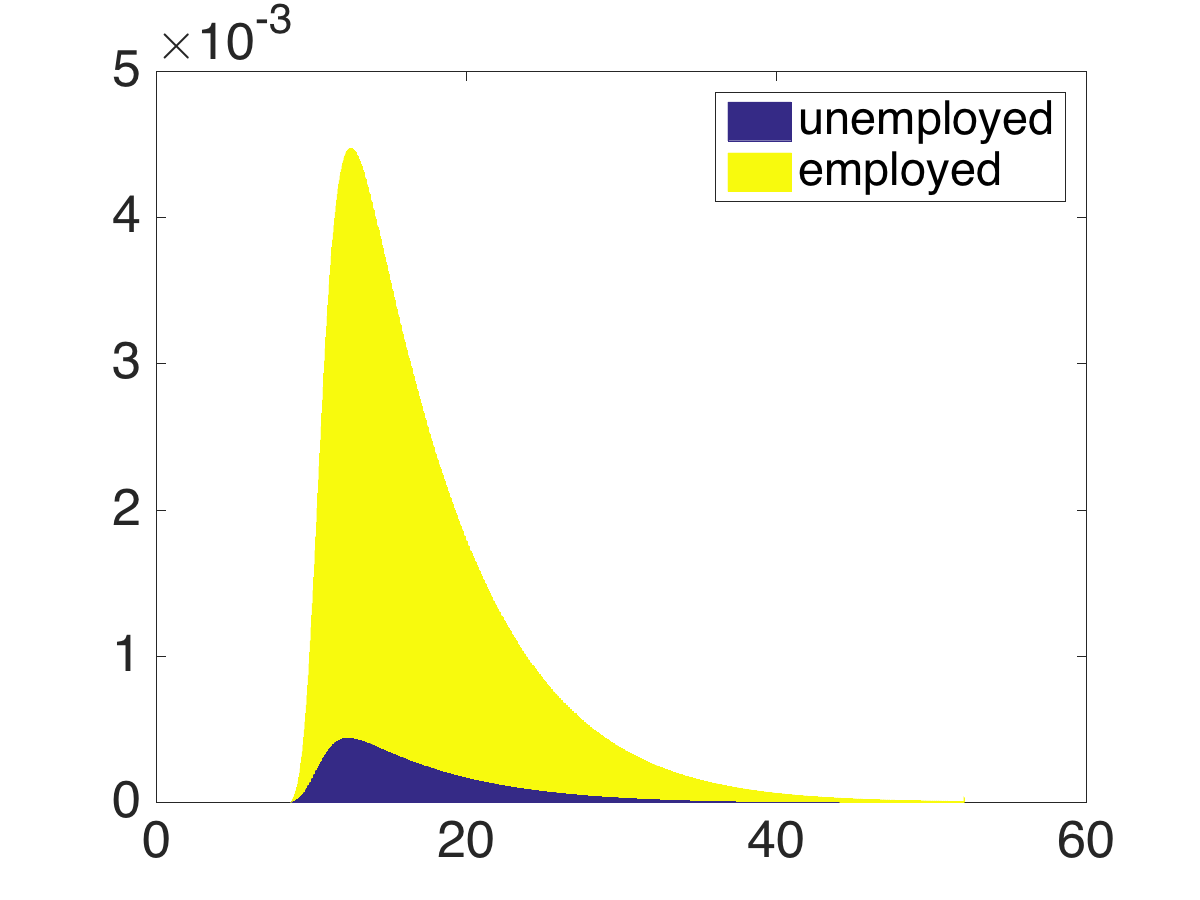
\includegraphics[width=\textwidth]{distribution3}
  \end{minipage}
\end{figure}
\ \ \ \ \ \ \  UI = 0.01 \ \ \ \ \ \ \ \ \ \ \ \ UI = 0.40 \ \ \ \ \ \ \ \ \ \ \ \ \ UI = 0.8
\end{frame}


\begin{frame}{The limitations}
  
  \begin{itemize}
  
  \item {The model's labor supply is exogenous. Thus, changing the unemployment benefits has no impact on labor supply or the transition probabilities.
} 
  \item {This contradicts empirical evidence: \citeauthor{decker} \cite{decker}.
  }
  \item{Endogenous labor matters: \citeauthor{mukoyama} \cite{mukoyama}.
  }

  \end{itemize} 
\end{frame}


\begin{frame}{Summary}
  
  \begin{itemize}
  
  \item {
Idiosyncratic risk affects aggregate variables.
  }

    \item {
Increasing unemployment benefits has distributional consequences. 
  } 

\item {
Welfare implications are unclear.
}





  \end{itemize} 
\end{frame}



\section{Welfare analysis of unemployment benefits}
\subsection{}
\begin{frame}{Welfare Analysis}
  \begin{itemize}
  \item {
  Which variable should we look at if we want to say consumers are better off? Output? Consumption?
  }
  \item {
  We want to measure somehow whether consumer welfare increased or not.
  }
  \item {
  But how to measure welfare? Can we compare the utility levels of consumers? And whose utility should we compare in a heterogeneous agent framework?
  }
  \end{itemize}
\end{frame}

\begin{frame}{Life-time Utility}
  \begin{itemize}
  \item {
  We calculate the life-time utility of each agent when the economy is in steady state. One time before the policy change and once after the policy change.
  }
  \item {
  Cannot compare two steady states directly. We need to take the transition into account.
  }
  \item {
  Calculating the exact transition path is troublesome. We follow the approximation by \citeauthor{sahin} \cite{sahin} which takes care of the idiosyncratic transition.
  }
    \begin{itemize}
    \item {
    Just place the agents in the first economy with their current assets into the second economy.
    }
    \end{itemize}
  \end{itemize}
\end{frame}

\begin{frame}{Welfare Analysis}
  \begin{itemize}
  \item {
  Now we can compare the utility level of the same agent before and after the policy change.
  }
  \item {
  Need to come up with a way to quantify the utility differences sensibly.
  }
  \item {
  We calculate a consumption and a cash equivalent of the policy change.
  }
  \end{itemize}
\end{frame}

\begin{frame}{Consumption Equivalent}
  \begin{itemize}

  \item {
  Permanent change of consumption by factor $\Delta$ that increases life-time
  utility by same amount as policy change:
  }
  \end{itemize}
  \begin{equation}
  U^{2}(e,k) = \mathbb{E}\sum_{t=0}^{\infty}\beta^{t}\frac{(c^{1}_{i,t}\Delta)^{1-\sigma}-1}{1-\sigma}\nonumber
  \end{equation}
  \begin{itemize}
  \item {
  If $ \Delta>1 $ agents prefer policy change $ (U^{2}) $, otherwise they do not want it.
  }
  \end{itemize}
\end{frame}

\begin{frame}{Consumption Equivalent}
  \centering{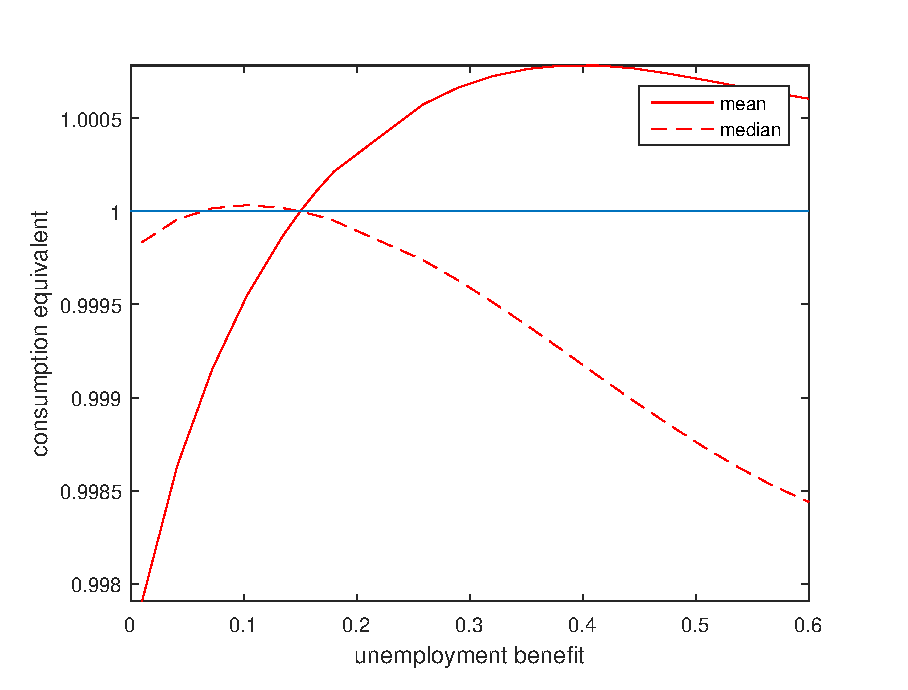
\includegraphics[scale=0.6]{cons_equiv}}
\end{frame}


\begin{frame}{Consumption Equivalent vs Wealth}
  \centering{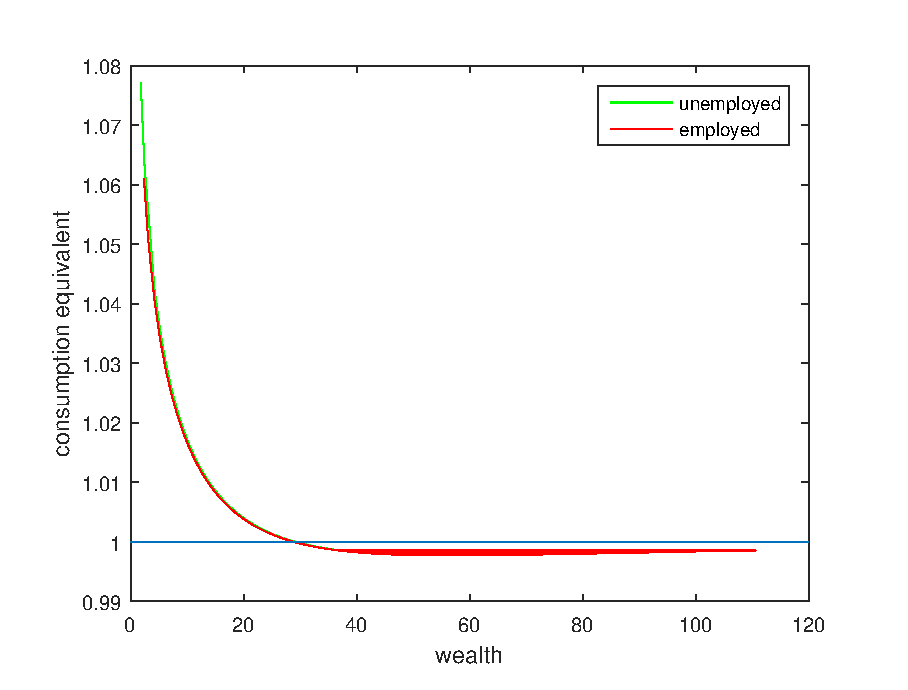
\includegraphics[scale=0.6]{cons_equiv_wealth}}
\end{frame}

\begin{frame}{Consumption Equivalent}
  \begin{itemize}
  
  \item {
  The consumption equivalent is biased towards poorer agents as relative increases for them are higher than for already-high consumption agents. Therefore, we need another measure.
  }
  \end{itemize}
\end{frame}

\begin{frame}{Cash Equivalent}
  \begin{itemize}
  \item {
  Transfer of $\Delta$ units of wealth in the first period
  }
  \end{itemize}
  
  \begin{equation}
  U^{2}(e,k) = U^{1}(e,k+\Delta) \nonumber
  \end{equation}
  
  \begin{itemize}
  \item {
  If $ \Delta>0 $ agents prefer the policy change $ (U^{2}) $, otherwise not.
  }
  \end{itemize}
\end{frame}

\begin{frame}{Cash Equivalent}
  \centering{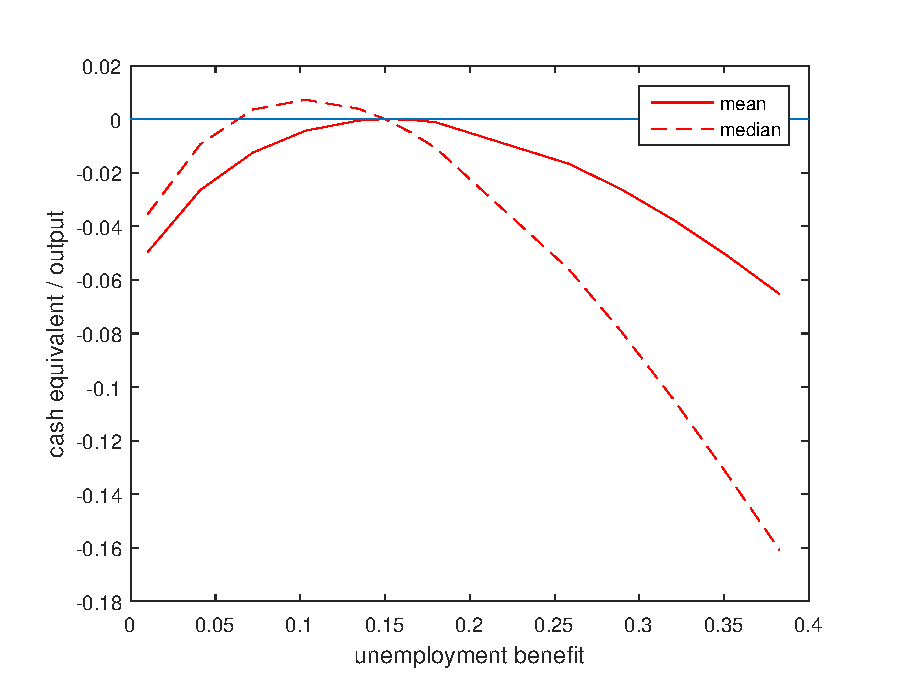
\includegraphics[scale=0.6]{cash_equiv}}
\end{frame}

\begin{frame}{Cash Equivalent}
  \centering{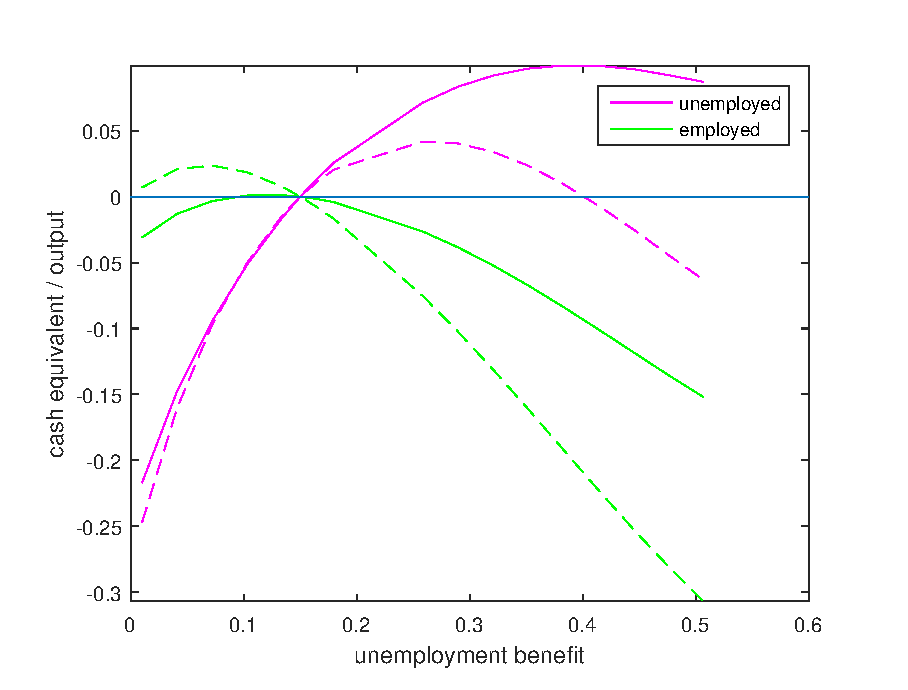
\includegraphics[scale=0.6]{cash_equiv_unemp_emp}}
\end{frame}

\begin{frame}{Summary}
  \begin{itemize}
  \item {
  Agents do not want full unemployment insurance although there is no moral hazard.
  }
  \item {
  Different groups in society want different policies. We did not find a policy reform that could make everyone better off with certainty.
  }
  \item {
  Of course, the model is not complete. A next step would be to endogenize the unemployment rate such that it reacts to changes in unemployment benefits.
  }
  \end{itemize}
\end{frame}


\section{The cost of the business cycle}
\subsection{}

\begin{frame}{Adding Aggregate uncertainty}
  \begin{itemize}

  \item {
  Aggregate uncertainty! Why?
  }

  \pause

  \item {
   Two productivity states: $z_t \in \{ 0.99, 1.01\}$.
  }

  \item {
  Two unemployment states. $U \in \{0.1, 0.04\}$.
  }



 \end{itemize}

\end{frame}

\begin{frame}{Problem}
  \begin{itemize}

  \item {
  The introduction of aggregate uncertainty makes the distribution of wealth changing over time.
  }

  \item {
  The capital distribution must be taken into account by the agents.  
  }

  \end{itemize}
\end{frame}

\begin{frame}{Solution}
  \begin{itemize}

  \item {
  There is no exact solution.
  }

  \item {
  \citeauthor{krussel_smith97} \cite{krussel_smith97} suggested an algorithm to solve the issue by an approximation.  
  }

  \item {
  They assume that the agents forecast prices by using the future mean of the wealth distribution.  
  }

  \item {
  The actual forecast is made for the future mean based on previous realizations using some Least Squares technique.  
  }

  \end{itemize}
\end{frame}

\begin{frame}{Algorithm}
  \begin{enumerate}
    \item {
    Draw shocks.  
    }

    \item {
    Guess initial coefficients for the forecasting rule.  
    }

    \item {
    Solve the individual problem.  
    }

    \item {
    Simulate the economy and take the sequence of the distributions.  
    }

    \item {
    Estimate new coefficients based on past realizations of the distribution and iterate until they converge. 
    }

  

   



  \end{enumerate}
   \pause
    Solution based on \citeauthor{soft} \cite{soft}.
    
\end{frame}

\begin{frame}{Results}
  \begin{itemize}
    \item {
    When it is solved you obtain the final sequence of capital distributions implied by the individual policy function.
    }

    \item {
    Use the coefficients of the regression to see if the forecasts coincide.
    }

       

  \end{itemize}

 \textrm{Good state forecast:}  \\
  \[ \ln{K_t} = 0.09 + 0.97\ln{K_{t-1}}; R^2 = 0.99 \]\\
\textrm{Bad state forecast:} \\
  \[ \ln{K_t} = 0.10 + 0.97\ln{K_{t-1}}; R^2 = 0.99 \]

\end{frame}

\begin{frame}{Aggregate uncertainty}
\centering{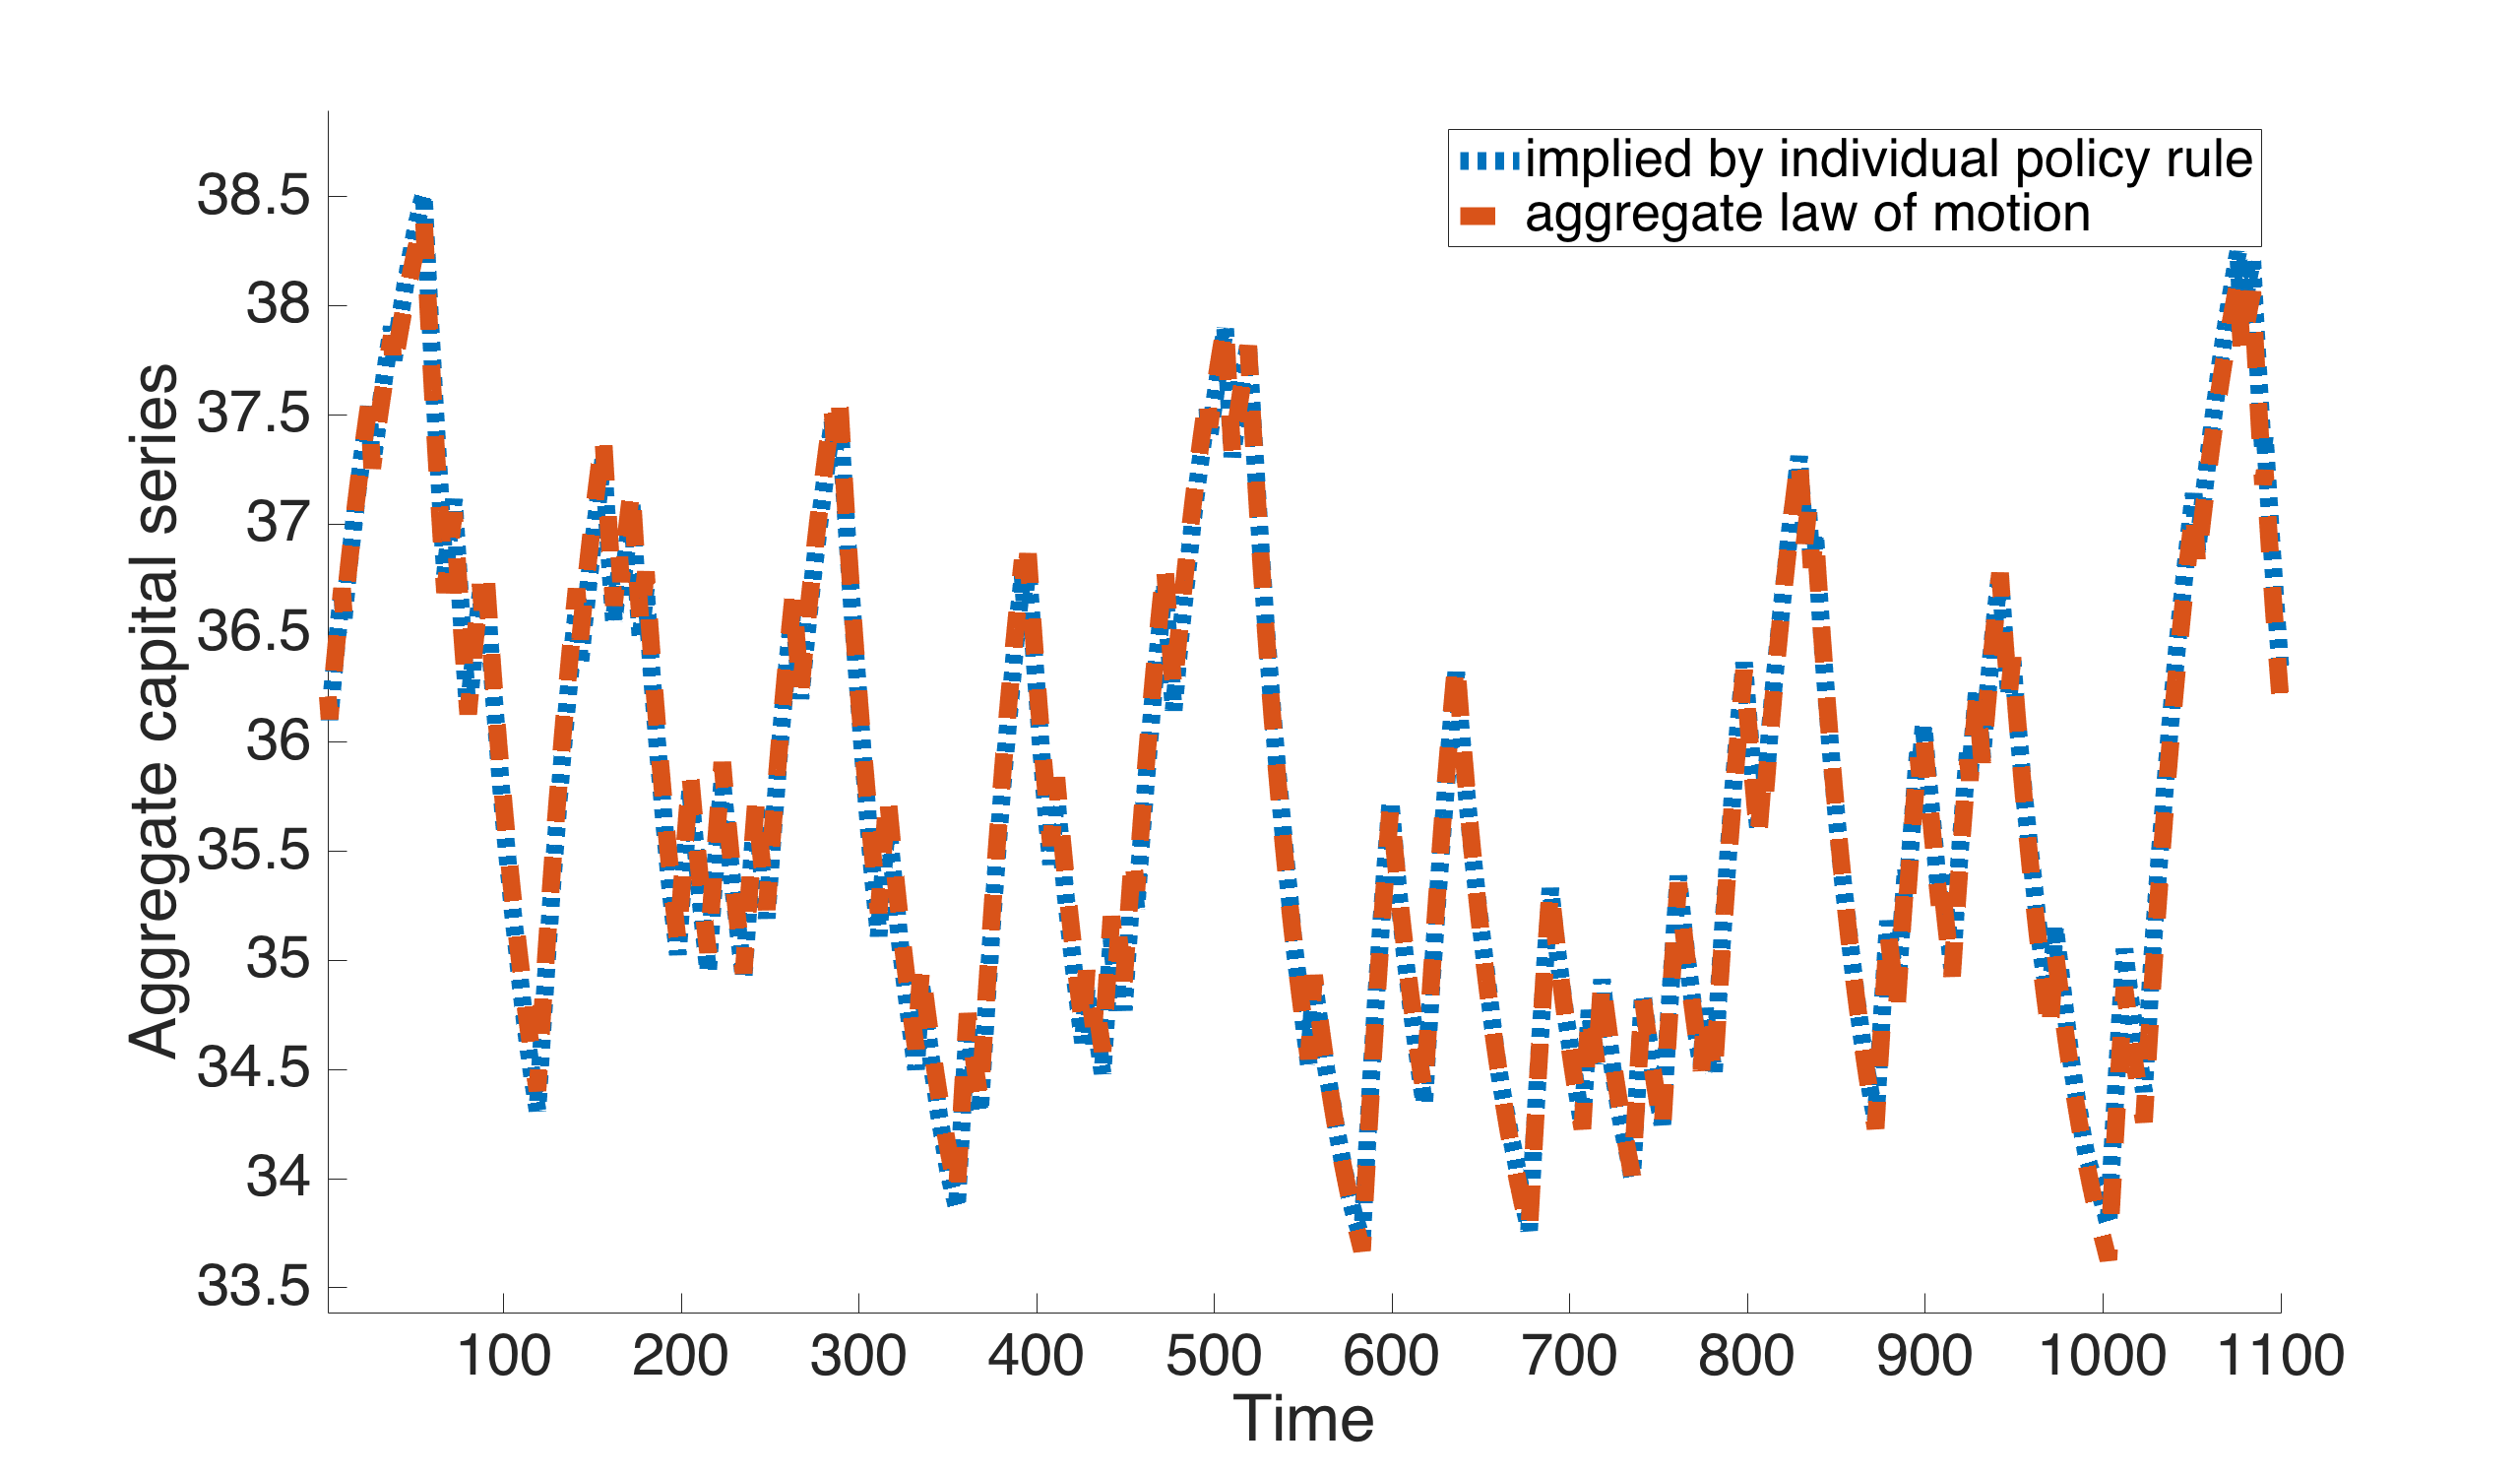
\includegraphics[width=12cm,height=7cm, keepaspectratio]{fig1}}
\end{frame}

\begin{frame}{Welfare loss of the business cycle}
  \begin{itemize}


  \item {
  Surpress Krussel - Smith algorithm such that the economy is initialy at the middle between good and bad state.
  }


  \item {
  Check if it converges to the steady state starting from a random and much higher aggregate demand level.  
  }

  \end{itemize}
\end{frame}

\begin{frame}{Welfare loss of the business cycle}{Convergence to steady state}
\centering{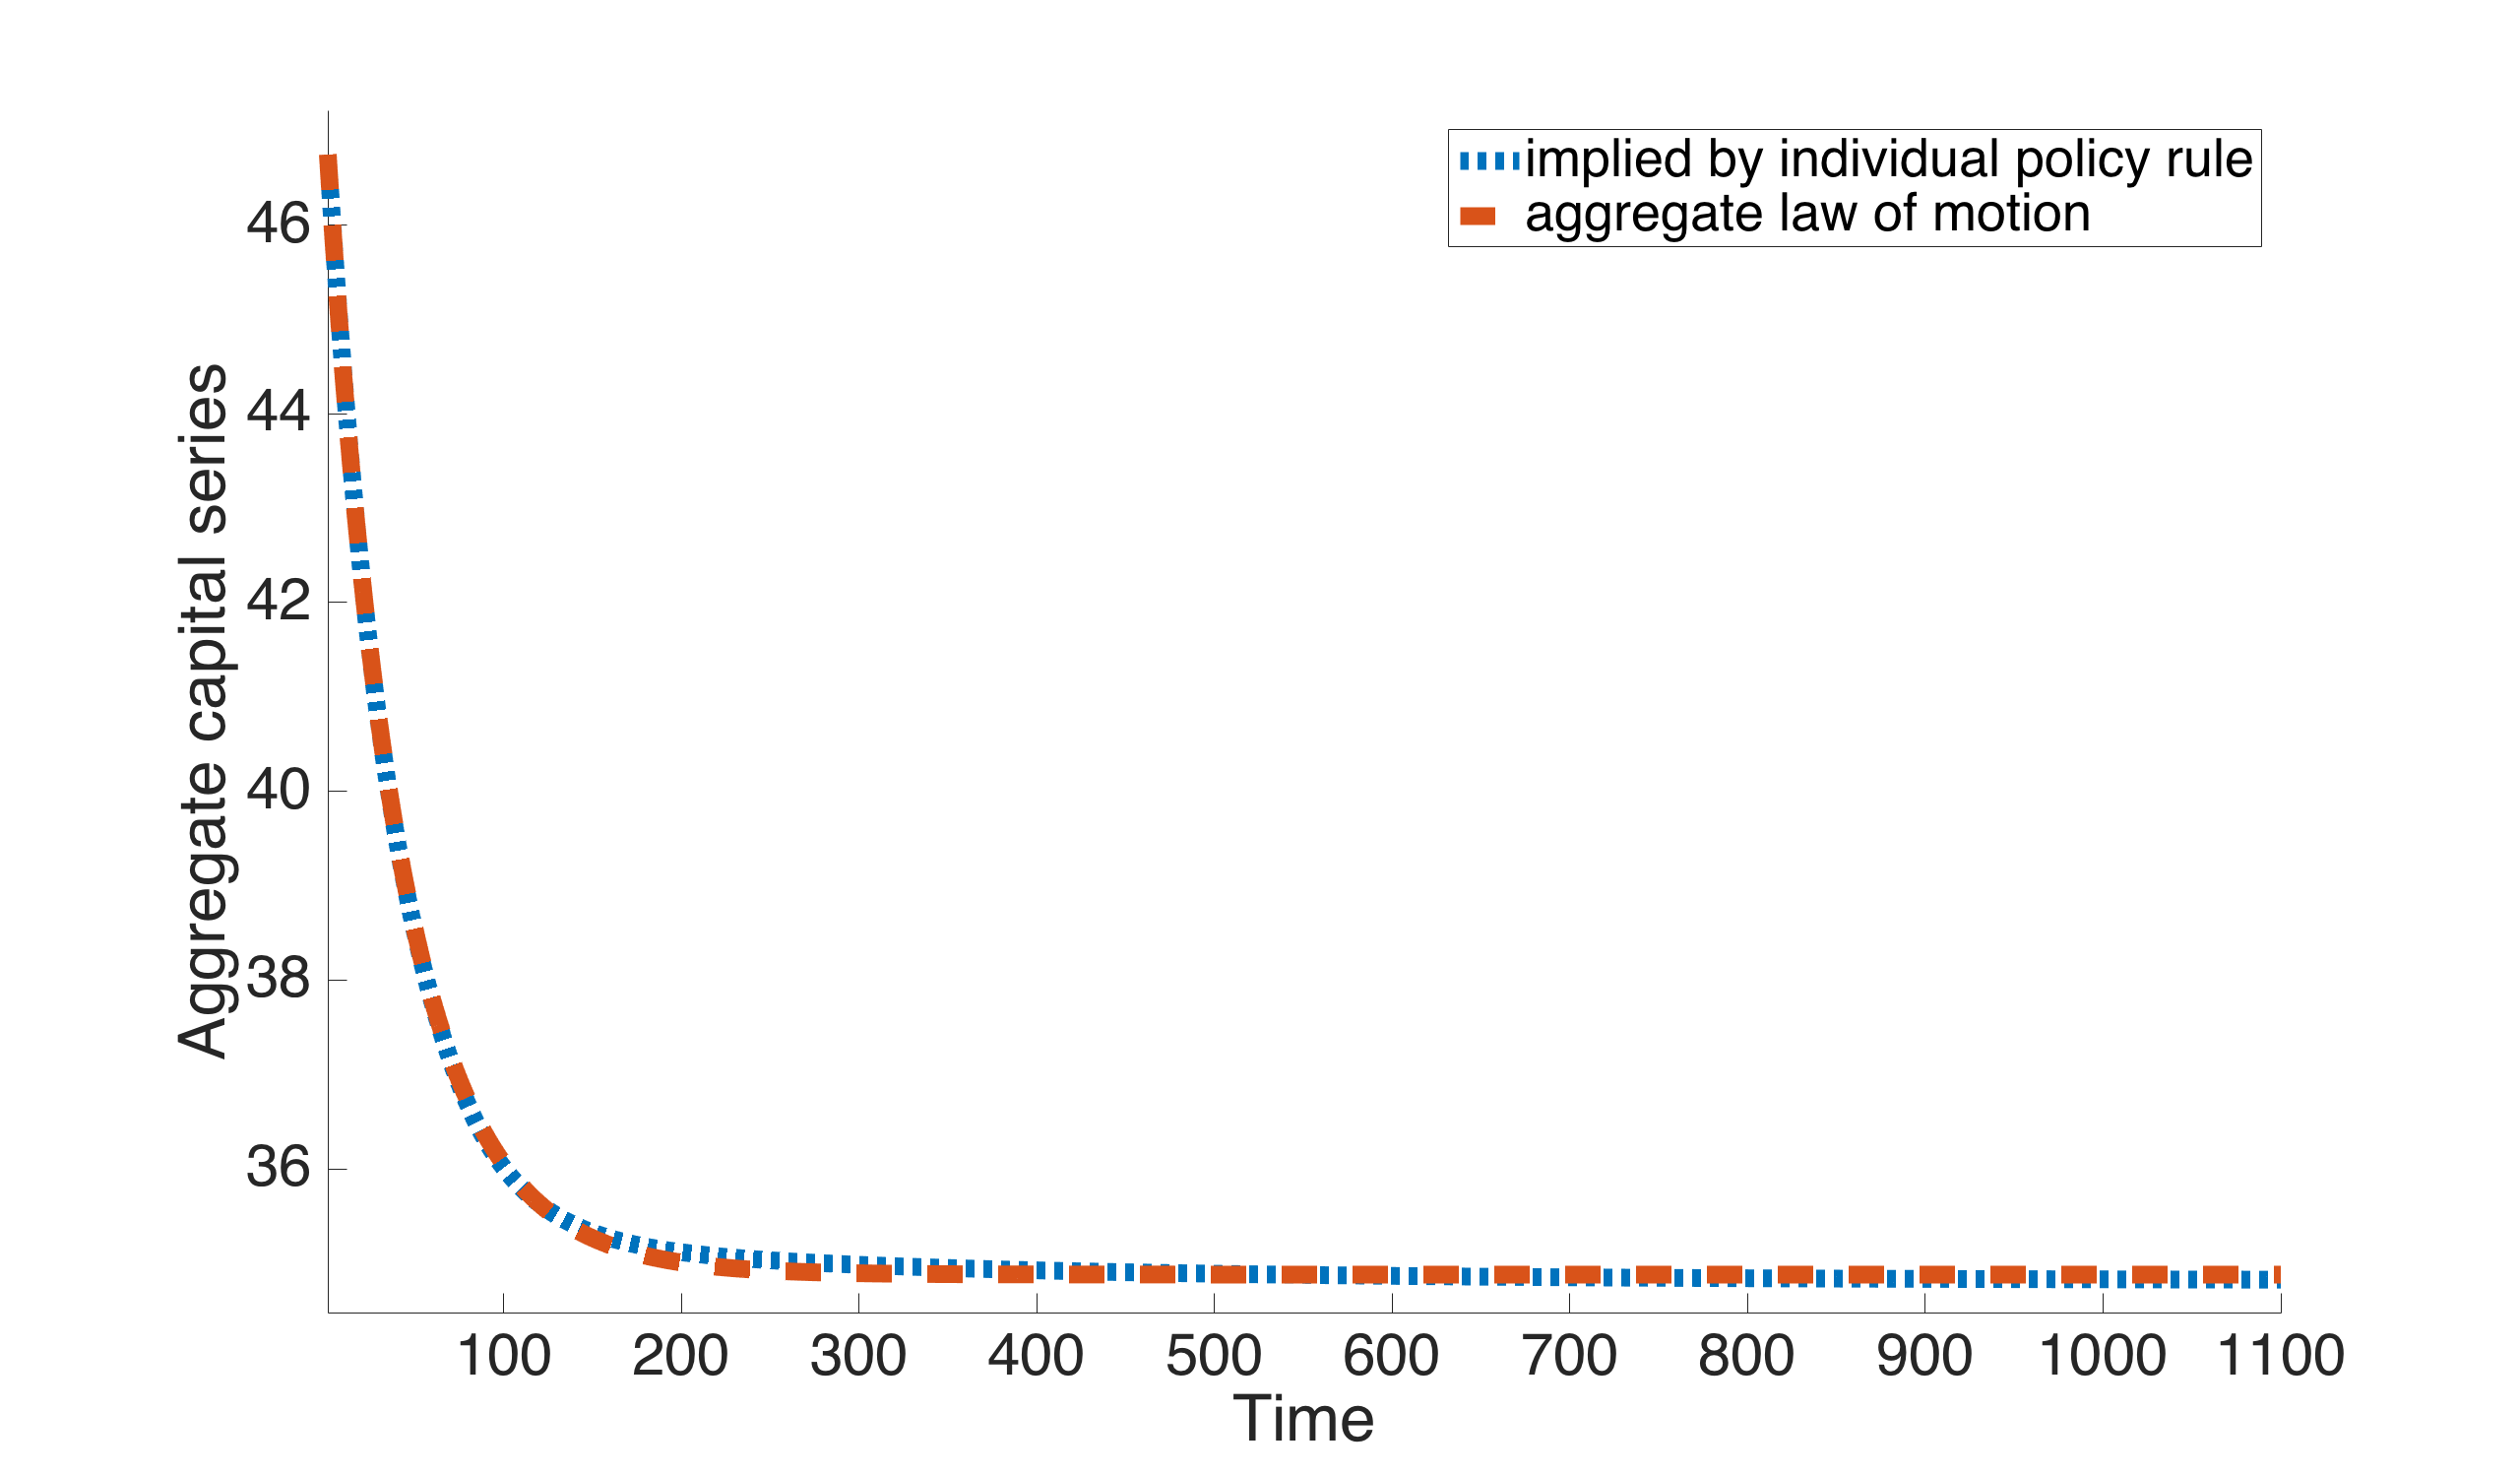
\includegraphics[width=12cm,height=6cm,keepaspectratio]{fig2}}
\end{frame}

\begin{frame}{Welfare loss of the business cycle}{Calculate lifetime utilities}
  \begin{itemize}

  \item {
  Solve the individual problem and the life-time utility for steady state. Calculate its value for all the consumers.
  }

  \item {
  Take the ergodic distribution and put it in aggregate economy framework. Solve the individual problem and calculate the \textbf{EXPECTED} lifetime utility. 
  }

  \[\textrm{Compare: }U^1(k_i, e_i) \textrm{ and } \mathbb{E}U^2(k_i, e_i, K^{ss}, z)\]

  \item {
  Calculate the consumption equivalent.  
  }

  \end{itemize}
\end{frame}

\begin{frame}{Results}
  \begin{itemize}

  \item {
  The median consumption equivalent is: 0.1603\%.
  }

  \item {
  The median personal disposable income for 2015 is \$30,240 (U.S. Bureau of the Census).
  }

  \item {
  The consumers would give up to \$48.47 per year or 13 $\cent$ per day to eliminate the business cycle.
  }

  \item {
  Similar results to \citeauthor{ks_99} \cite{ks_99}. 
  }

  \end{itemize}
\end{frame}

\begin{frame}{Winners and losers from the business cycle}
\centering{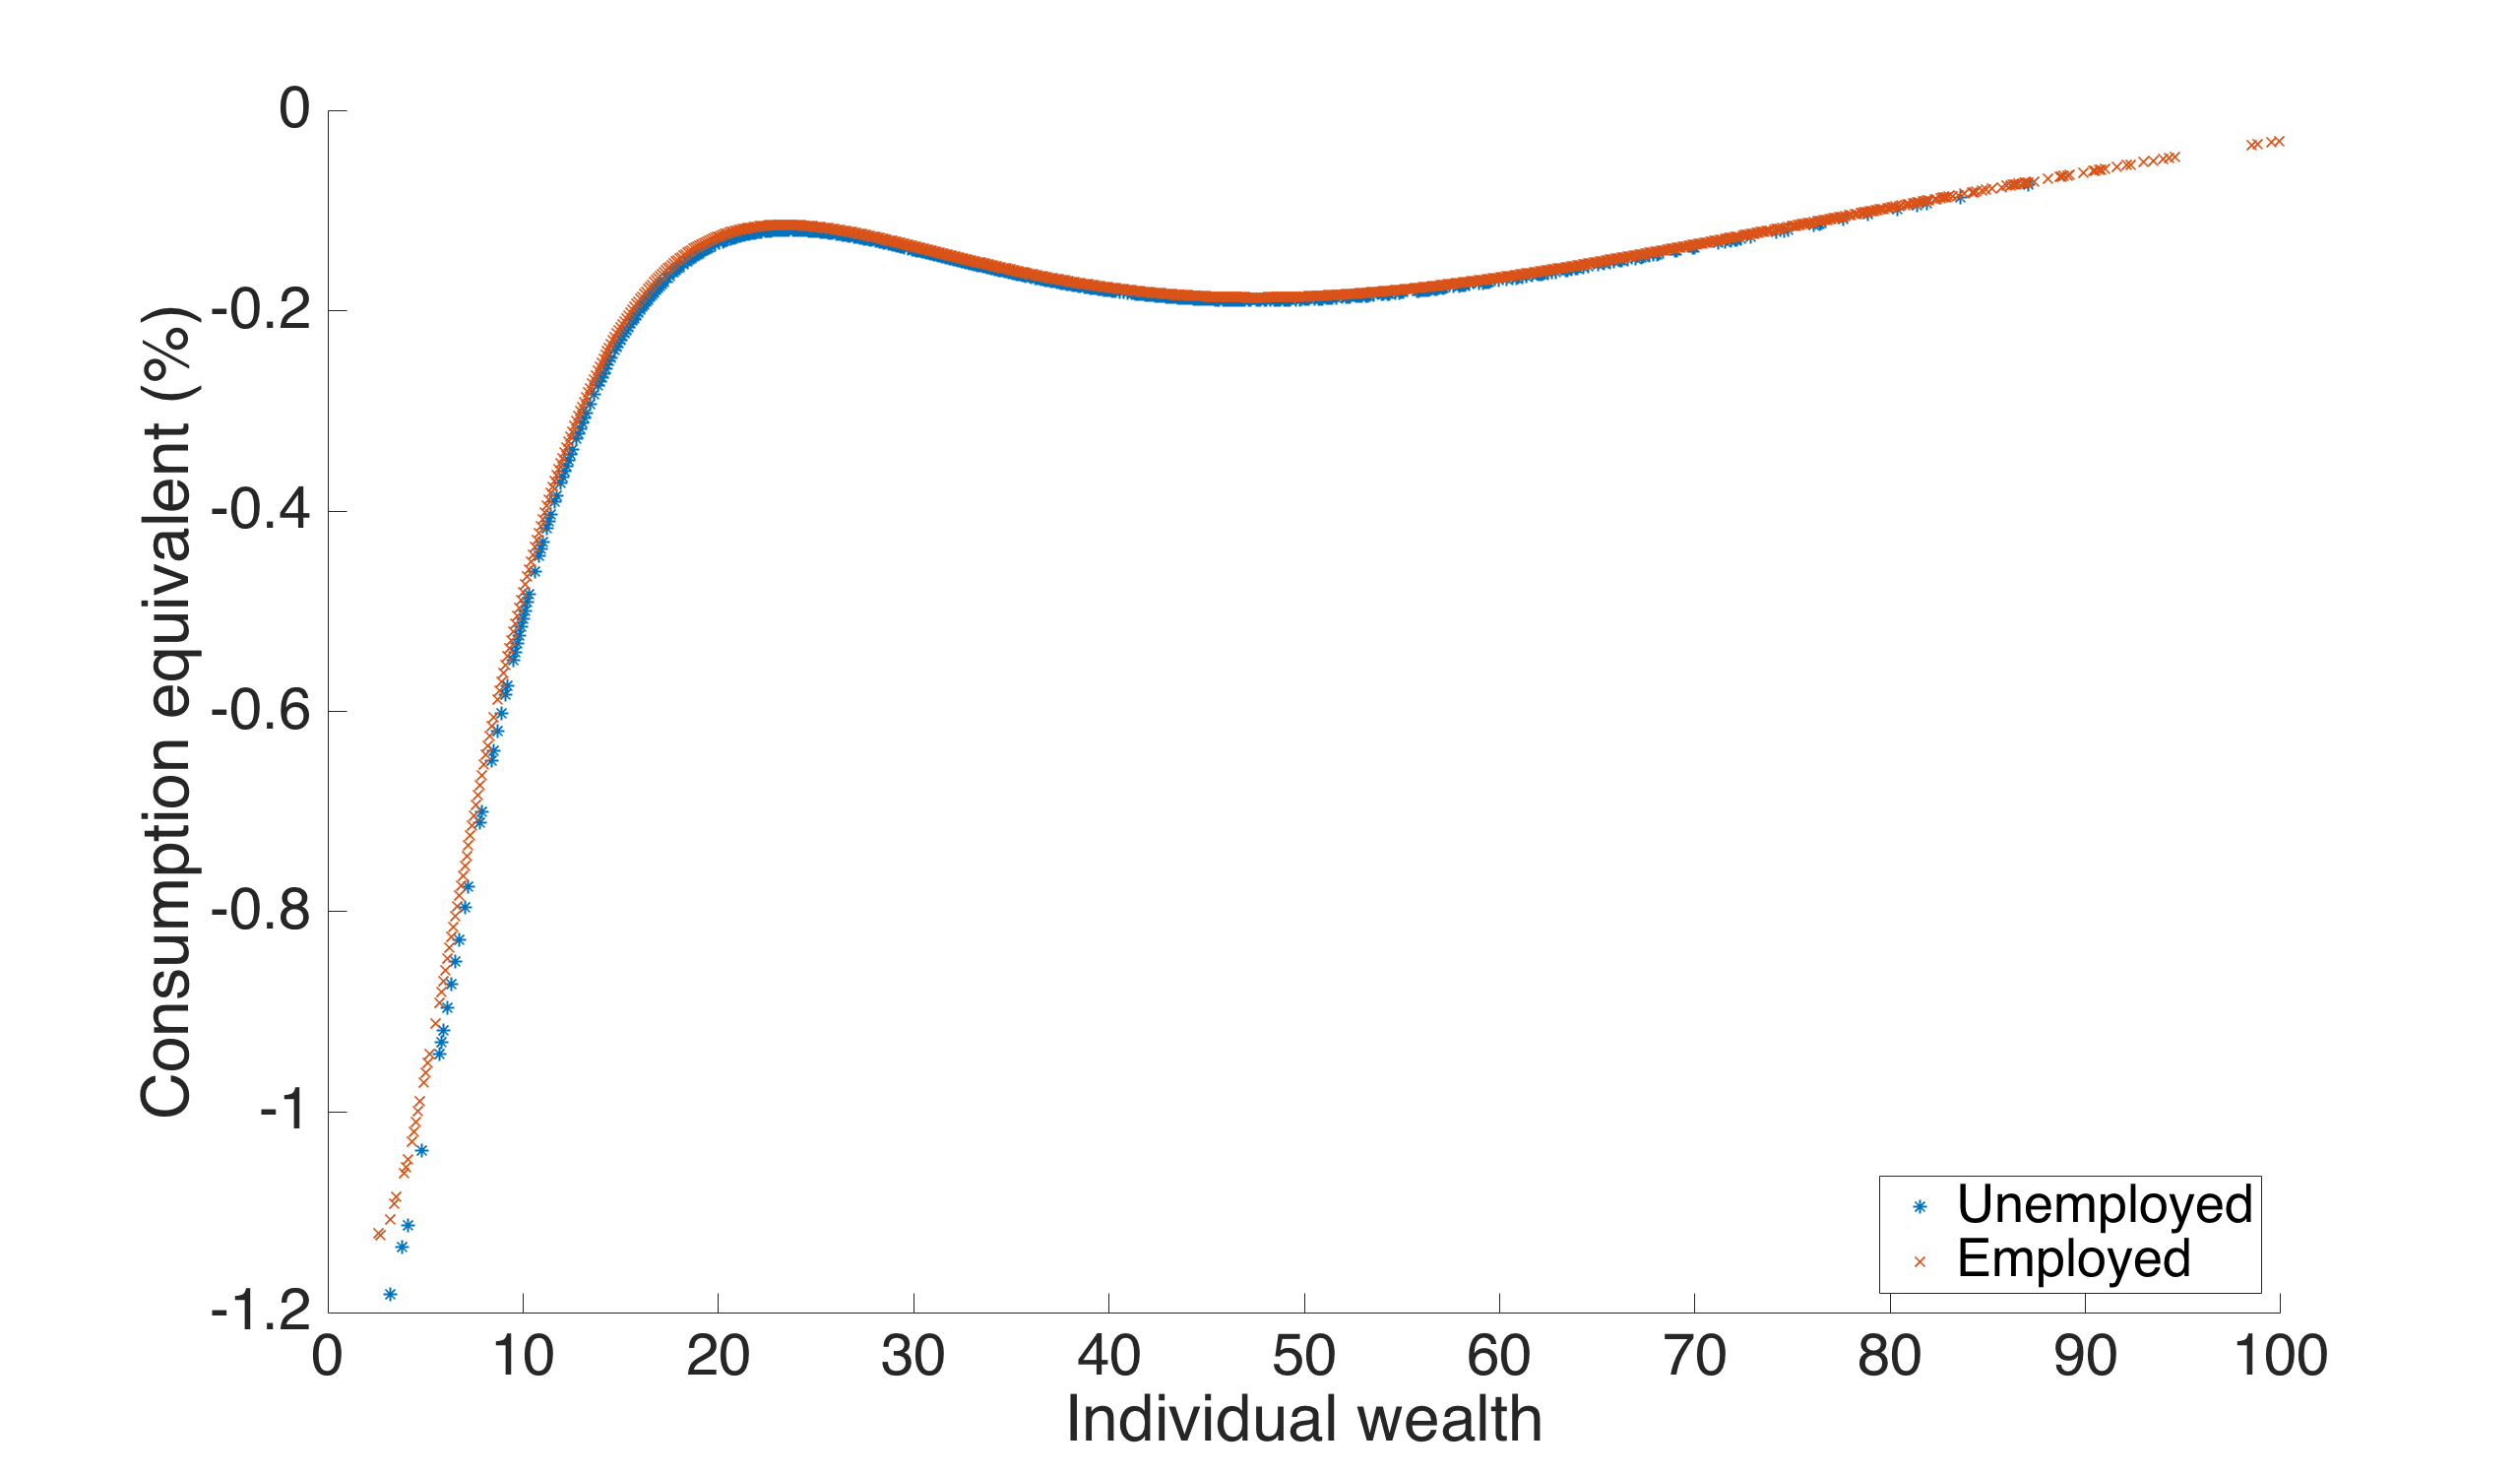
\includegraphics[width=40cm,height=6.5cm,keepaspectratio]{cons_equiv_agg}}
\end{frame}

\section{Numerical problems}
\subsection{}
\begin{frame}{Another application of Krussel - Smith}{Transition between two steady states for 10k individuals}
\centering{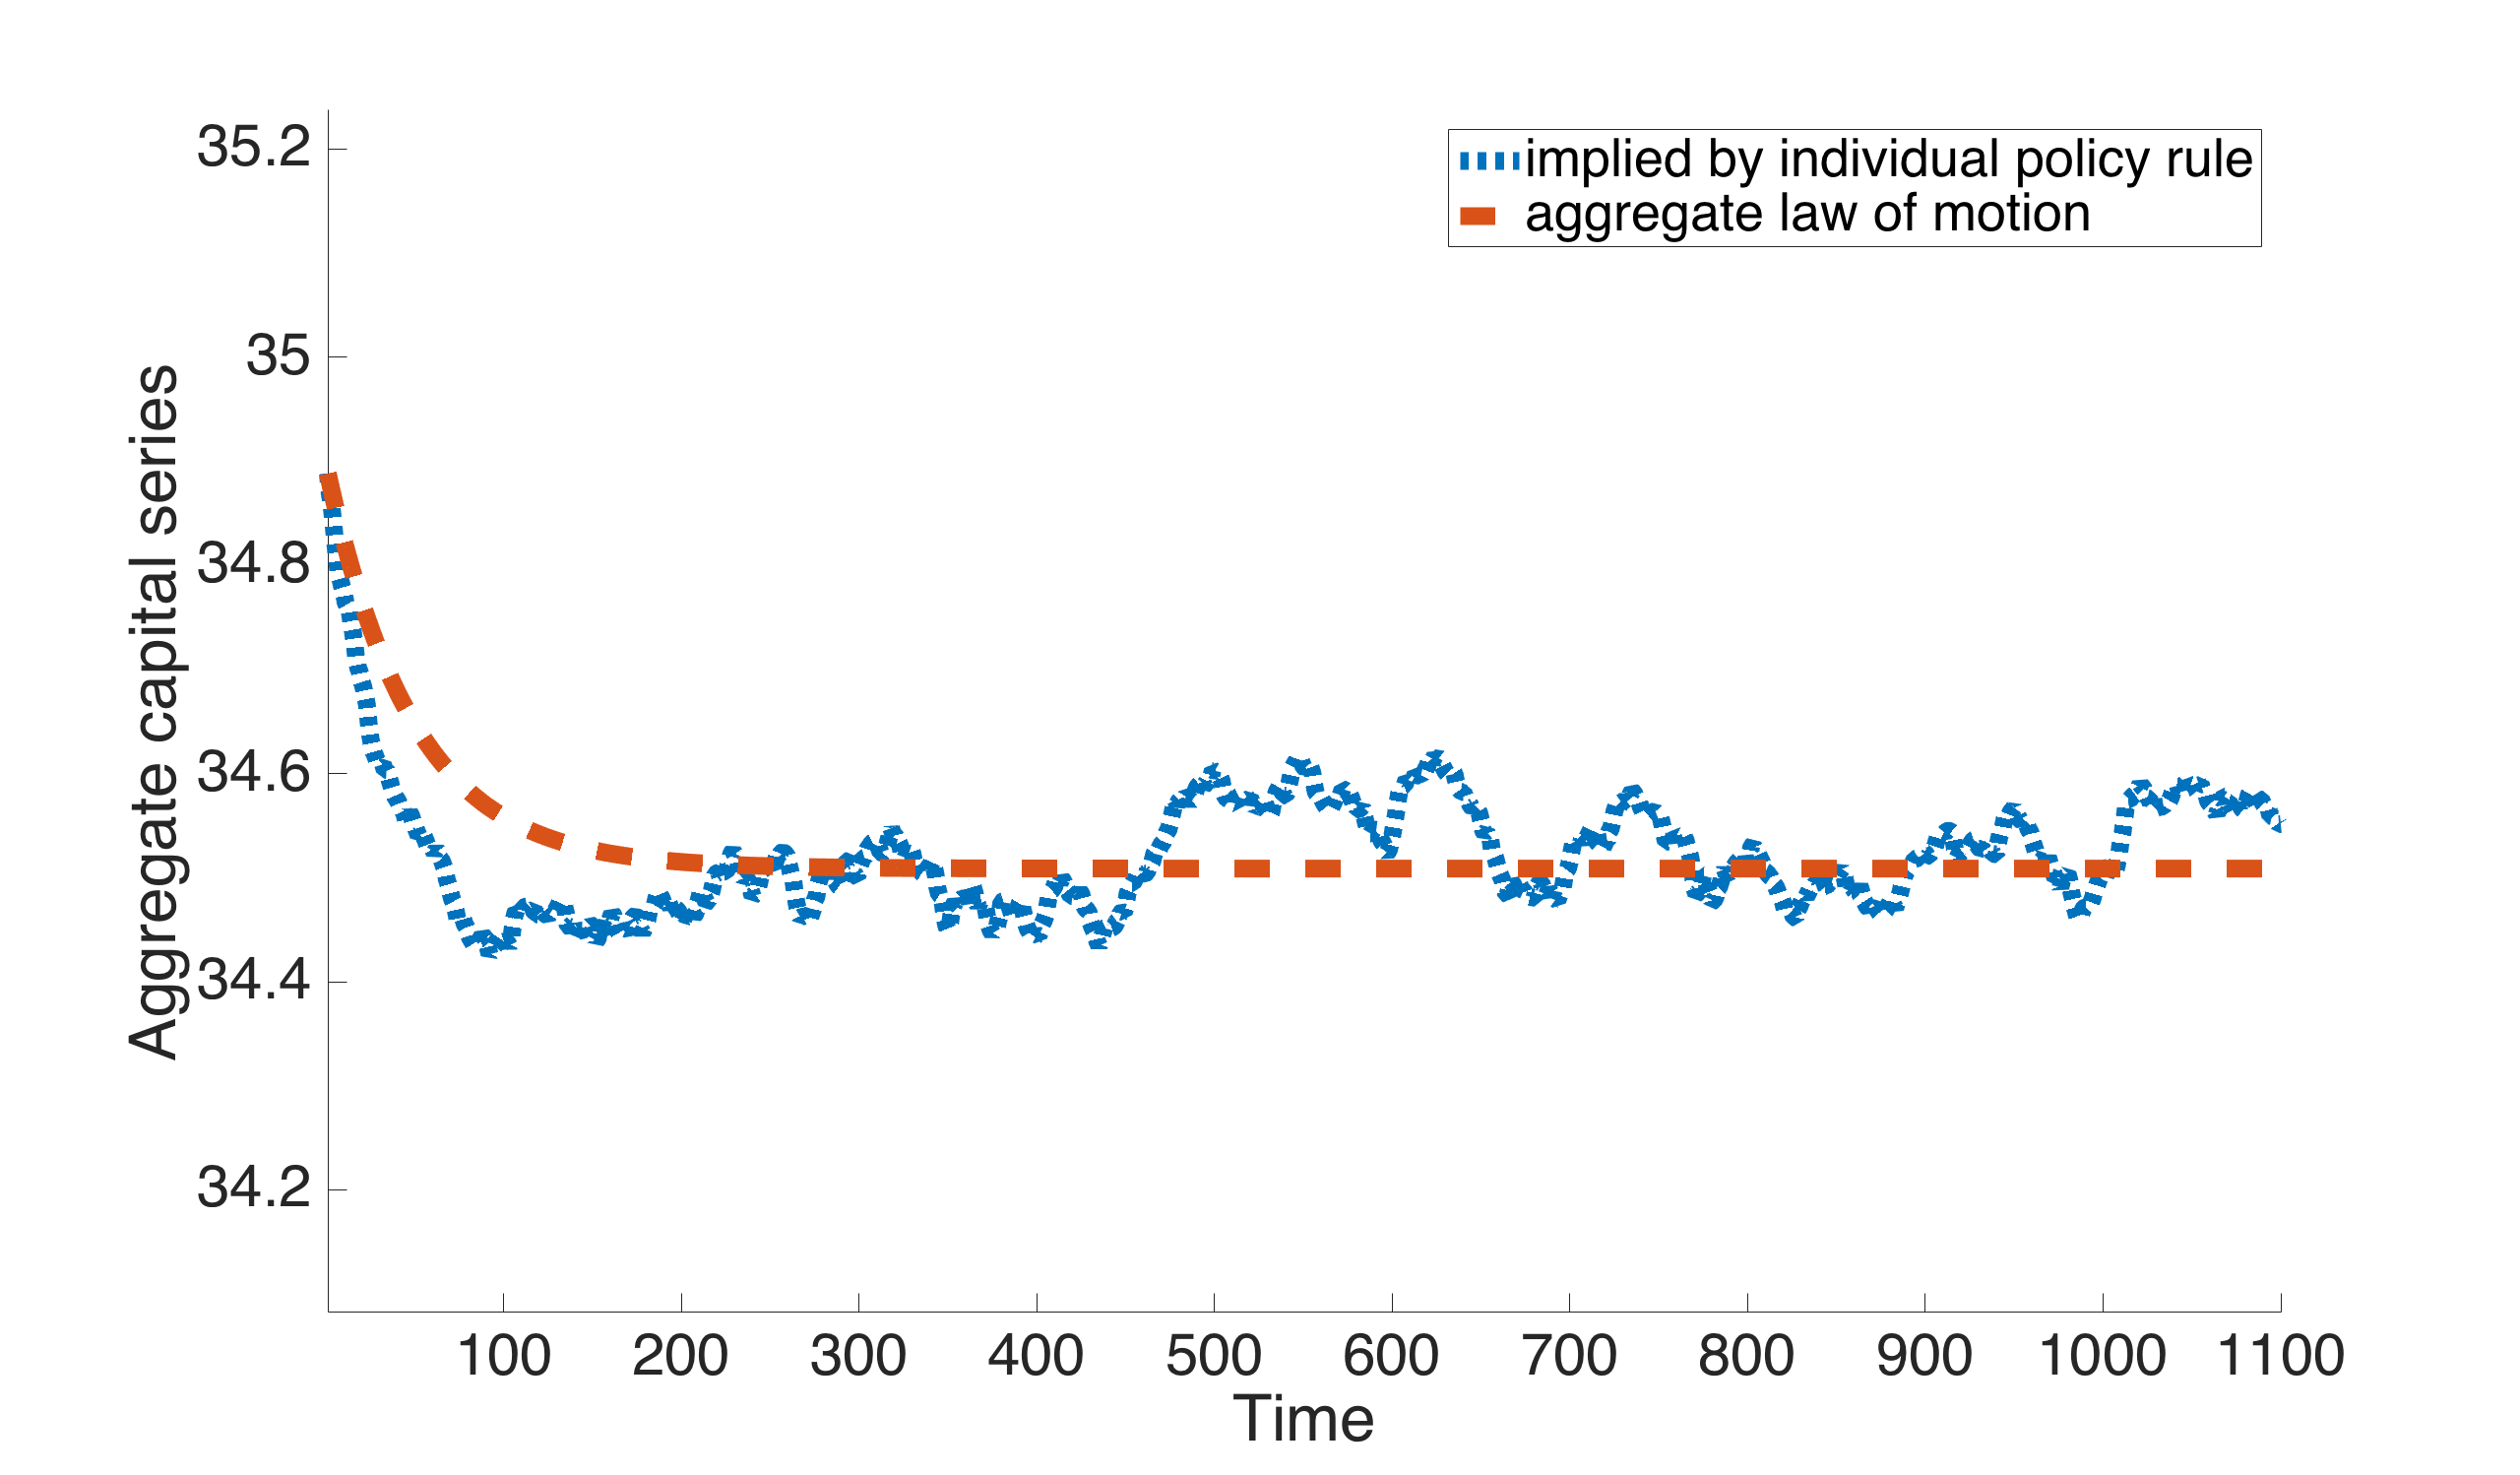
\includegraphics[width=12cm,height=6cm,keepaspectratio]{fig3}}
\end{frame}

\begin{frame}{Another application}{Transition between two steady states for 100k individuals}
\centering{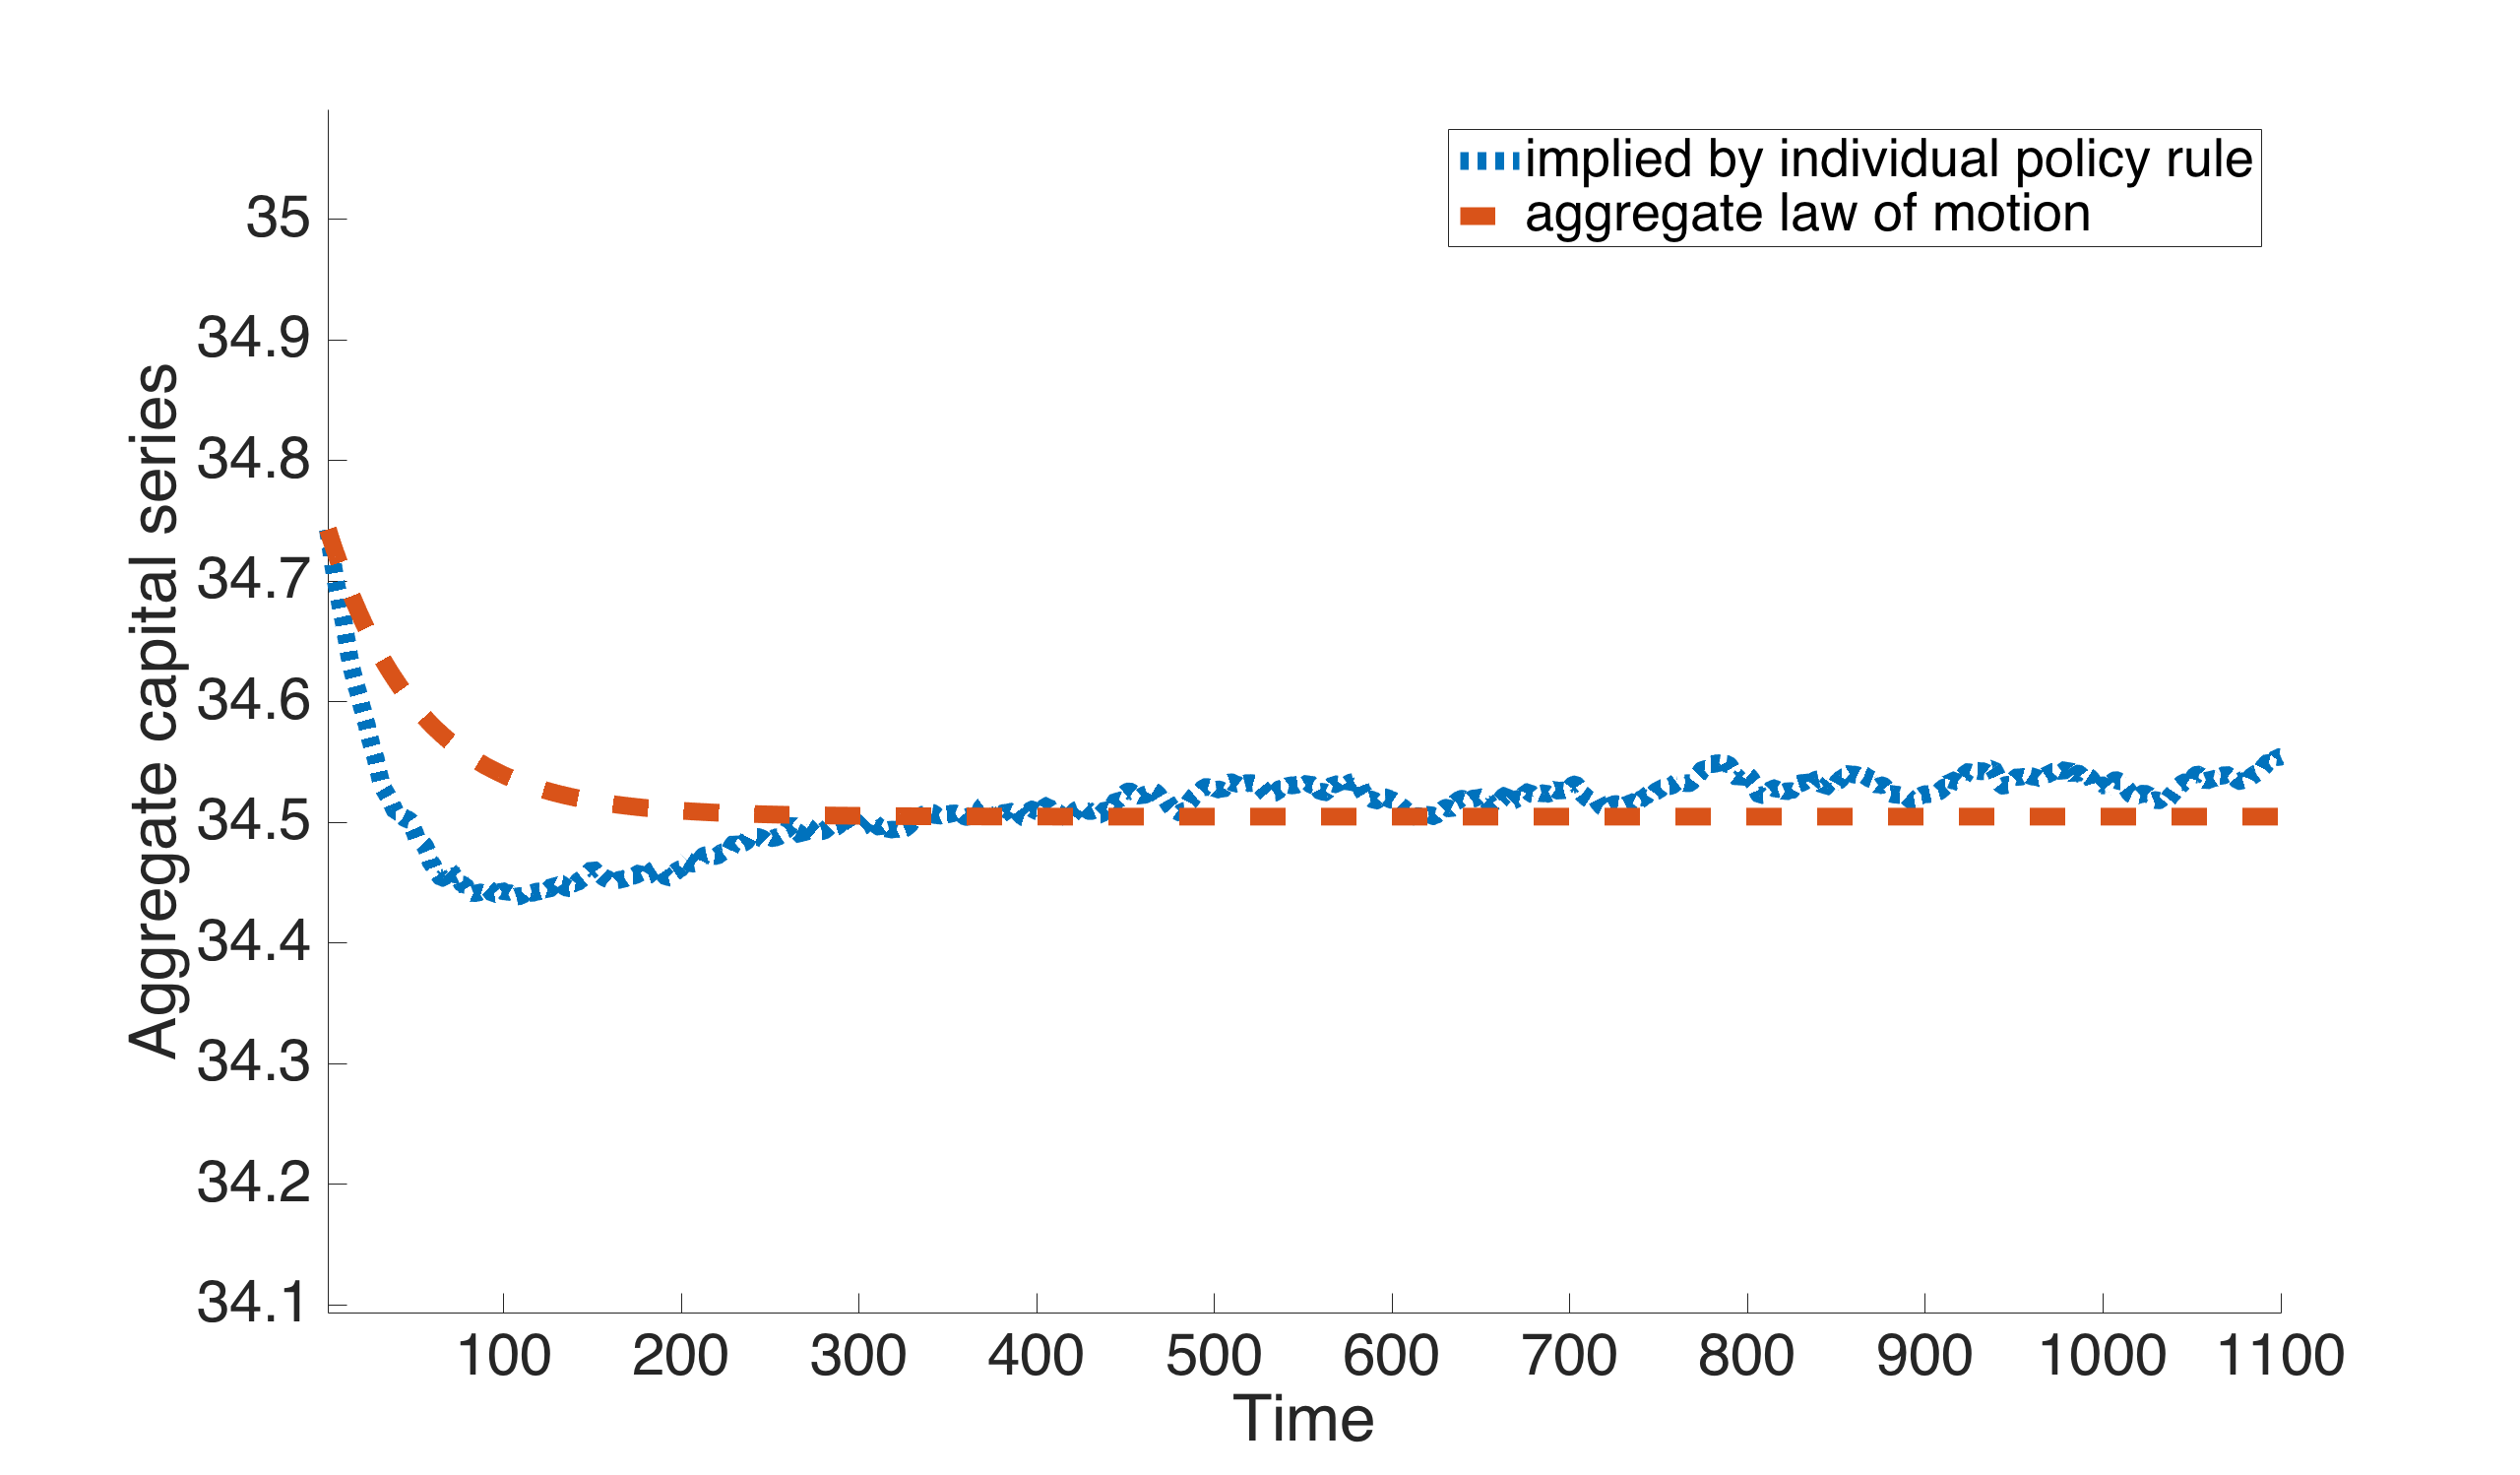
\includegraphics[width=12cm,height=6cm,keepaspectratio]{fig4}}
\end{frame}

\begin{frame}{Another application}{Transition between two steady states for histogram method}
\centering{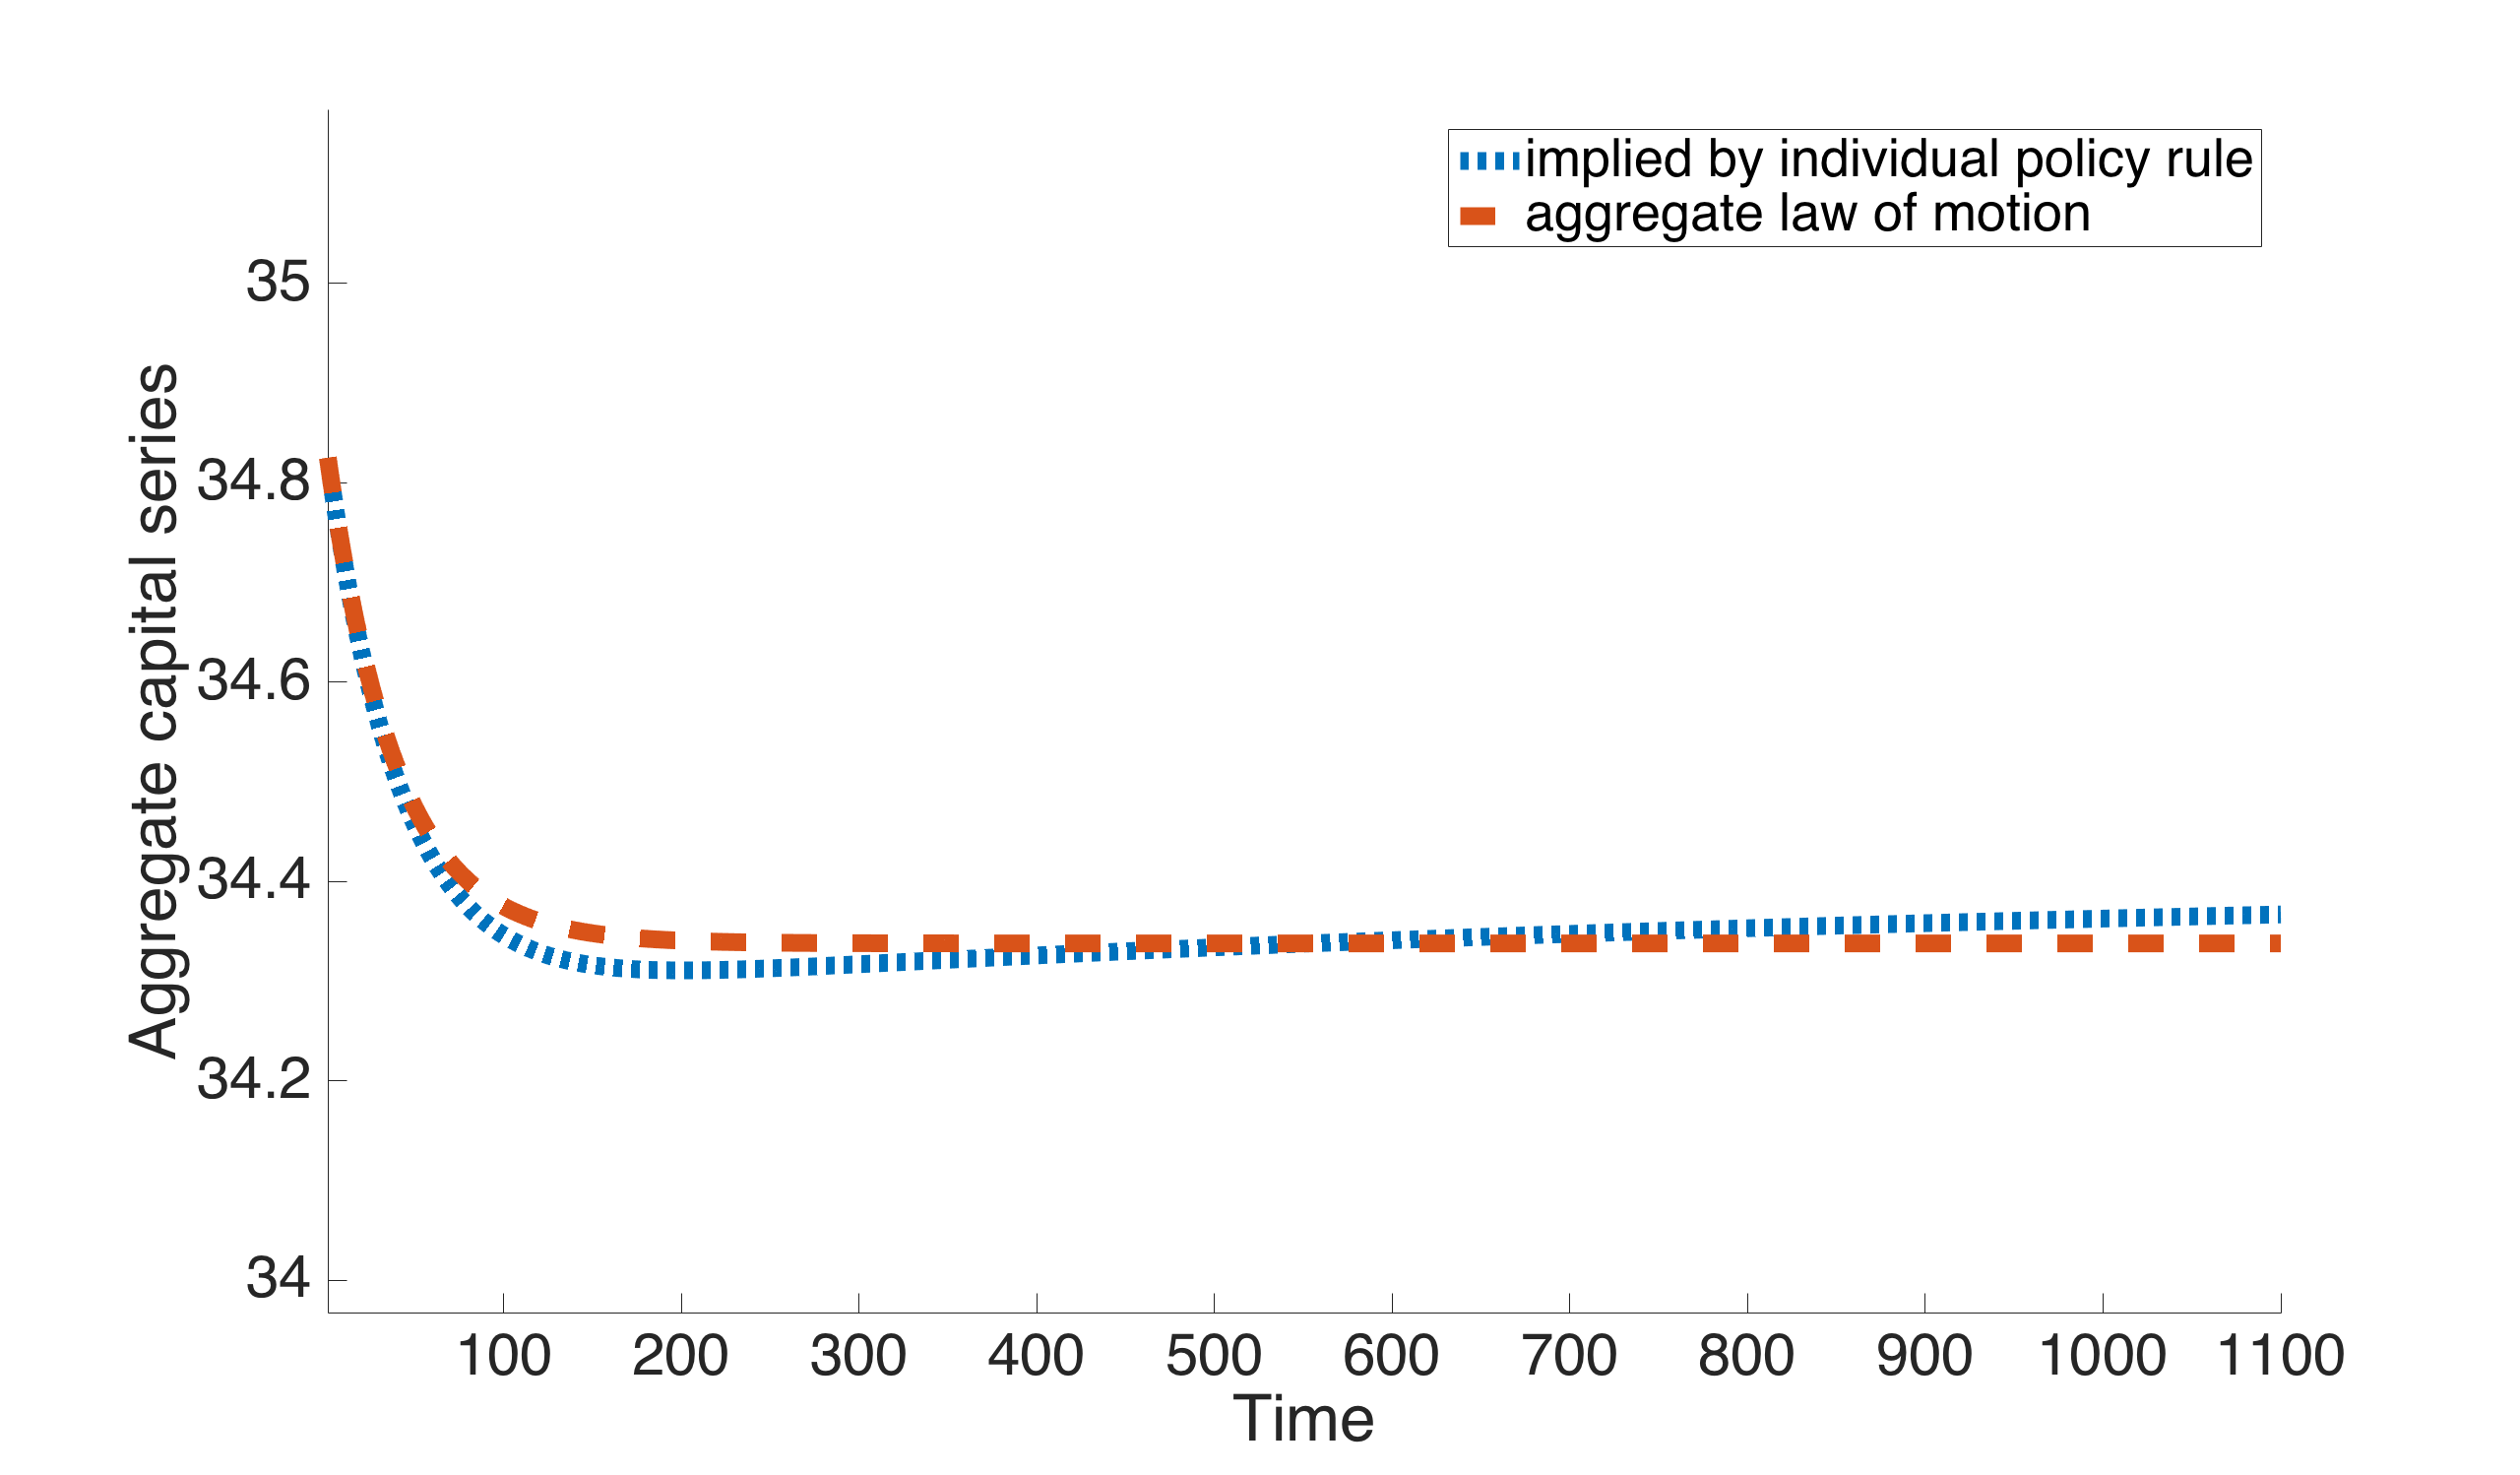
\includegraphics[width=12cm,height=6cm,keepaspectratio]{fig5}}
\end{frame}

\begin{frame}{Numerical problems and solutions}
  \begin{itemize}

  \item {
  How to calibrate?
  }

  

  \item {
  How to choose state space?

  \begin{itemize}
    \item Boundaries
    \item {
    Precision  
    }
    \item {
    Position  
    }
  \end{itemize}

  }

 
  \item {
  How to solve the individual problem?  
  }
  
  
  \item {
  How to find the ergodic distribution?  
  }
 



  \end{itemize}
\end{frame}


\section{Conclusion}
\begin{frame}{Conclusion}
  \begin{enumerate}

  \item {
  Government policies could influece the economy significantly!
  }

  \item {
  There is no Pareto improvement!
  }

  \item {
  Aggregate uncertainty doesn't matter much!
  }

  \end{enumerate}
\end{frame}

\appendix

\begin{frame}[allowframebreaks]{References}

\printbibliography
\end{frame}

\end{document}